\section*{} 
\begin{center}
    \Large\textbf{APPENDIX}
\end{center}

\noindent The code and dataset are publicly available at: 
\url{https://github.com/JonathanZha47/PadBen-Paraphrase-Attack-Benchmark}


\appendix

\section{Overall Data Processing}
\label{Appendix_A}

The experiment utilizes 16,233 human-authored sentences sourced from three established datasets following the pipeline shown in Figure~\ref{fig:preprocessing}:
\begin{itemize}
    \item \textbf{MRPC} (Microsoft Research Paraphrase Corpus) \cite{dolan2005automatically}
    \item \textbf{HLPC} (Human-Like Paraphrase Corpus)\cite{lau2024understandingeffectshumanwrittenparaphrases}
    \item \textbf{PAWS} (Paraphrase Adversaries from Word Scrambling)\cite{paws2019naacl}
\end{itemize}

\subsection{MRPC Processing}
The Microsoft Research Paraphrase Corpus (MRPC) \cite{dolan2005automatically} is a widely-used benchmark dataset for paraphrase detection, containing sentence pairs extracted from online news sources with human annotations indicating semantic equivalence. For dataset construction, only verified paraphrase pairs (\texttt{label == 1}) are extracted, utilizing \texttt{sentence1} as human original text and \texttt{sentence2} as human paraphrased text. This filtering ensures high-quality semantic equivalence relationships while maintaining the news domain characteristics.

\subsection{PAWS Processing}
The Paraphrase Adversaries from Word Scrambling (PAWS) dataset \cite{paws2019naacl} is specifically designed to challenge paraphrase identification systems with adversarial examples. The PAWS-QQP version is adopted, utilizing the \texttt{labeled\_final} subset and extracting only verified paraphrase pairs (\texttt{label == 1}), treating \texttt{sentence1} as human original text and \texttt{sentence2} as human paraphrased text.

\subsection{HLPC Processing}
The Human \& LLM Paraphrase Collection (HLPC) \cite{lau2024understandingeffectshumanwrittenparaphrases} is a comprehensive dataset aggregating paraphrase data from multiple established sources. The generated variants of HLPC are considered outdated since they mainly use GPT-2-XL as main language model. Hence, only \texttt{originalSentence1} and \texttt{originalSentence2} are utilized to extract high-quality human paraphrase pairs.

\subsection{Preprocessing}
Given the potential overlap between datasets (particularly between HLPC and MRPC), a systematic deduplication process is implemented to prevent data leakage.
\begin{figure}[t]
    \centering
     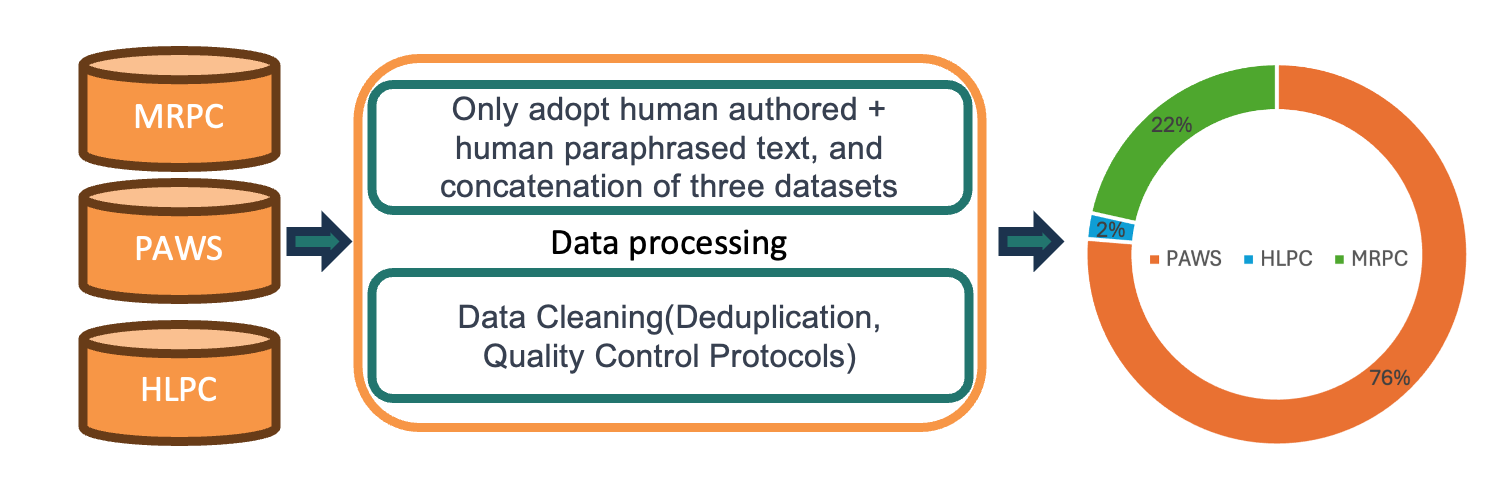
\includegraphics[width=\textwidth]{figures/preprocessing.png}
    \caption{The complete integration of HLPC, MRPC, and PAWS datasets follows a systematic pipeline that encompasses data loading, standardization, quality control, and deduplication.}
    \label{fig:preprocessing}
\end{figure}
\subsubsection{Quality Control Protocols}
\begin{enumerate}
    \item \textbf{Text Length Validation}: Remove entries with texts shorter than 10 characters or longer than 1000 characters
    \item \textbf{Encoding Validation}: Ensure proper UTF-8 encoding and remove entries with encoding issues
\end{enumerate}

\subsubsection{Similarity-Based Duplicate Detection}

TF-IDF vectorization combined with cosine similarity is employed to identify near-duplicate content across the combined dataset:

\begin{equation}
\text{Similarity}(t_i, t_j) = \frac{\mathbf{v}_i \cdot \mathbf{v}_j}{|\mathbf{v}_i||\mathbf{v}_j|}
\end{equation}

where $\mathbf{v}_i$ and $\mathbf{v}_j$ are TF-IDF vectors for texts $t_i$ and $t_j$.

\begin{algorithm}[H]
\caption{Deduplication Process}
\label{algo:deduplication}
\begin{algorithmic}[1]
\STATE Compute TF-IDF vectors for all \texttt{human\_original\_text} entries
\STATE Calculate pairwise cosine similarities
\FOR{each text pair $(t_i, t_j)$ where $\text{Similarity}(t_i, t_j) > \theta$}
    \STATE Identify as potential duplicate
    \STATE Retain entry with higher dataset priority: PAWS > MRPC > HLPC
    \STATE Mark duplicate for removal
\ENDFOR
\STATE Remove identified duplicates from combined dataset
\end{algorithmic}
\end{algorithm}

The threshold $\theta$ is set to 0.85 to ensure all adopted human-authored texts are unique.

\section{Intrinsic Mechanisms of Paraphrase Attacks}

\subsection{Experiment 1: Semantic Equivalence versus Paraphrasing in Representation Space}
\label{app:experiment1}

\subsubsection{Research Objective}
In this experiment, the primary goal is to verify whether Hypothesis 1 holds: that paraphrasing induces a distinct semantic transformation, differing from text generated via ``semantic equivalence'' prompting. This is assessed by comparing the embedding spaces of LLM-paraphrased and LLM-generated texts.

\subsubsection{Data Preparation}

Human-authored original sentences were collected from three established paraphrase datasets, following the preprocessing pipeline shown in Figure~\ref{fig:preprocessing}.

After applying quality control and deduplication procedures (detailed in Appendix~\ref{Appendix_A}), 16,233 unique human-authored sentences were obtained that serve as the foundation for generating the other two text categories.

\paragraph{LLM-Generated Text Creation}
\label{app:experiment1_llm_generated}
Using the 16,233 human-authored sentences as source material, semantically equivalent sentences were generated through LLM prompting. Unlike paraphrasing, this generation process aims to preserve the original meaning and structure without explicit rewording. The following semantic equivalence prompt was employed:

\begin{quote}
\small
\texttt{Given the following sentence, generate a new sentence that is semantically equivalent, preserving the original meaning and structure as closely as possible. Do not paraphrase or reword unnecessarily.}

\texttt{\{text\}}

\texttt{Generated sentence:}
\end{quote}

\paragraph{LLM-Paraphrased Text Creation}
\label{app:experiment1_paraphrased}
From the same 16,233 human-authored sentences, paraphrased versions were generated using explicit paraphrasing instructions. The paraphrasing prompt was:

\begin{quote}
\small
\texttt{Please paraphrase the following text while maintaining its original meaning:}

\texttt{\{text\}}

\texttt{Paraphrased text:}
\end{quote}

\subsubsection{Experimental Significance}
The experimental framework addresses two critical hypotheses:
\begin{itemize}
    \item \textbf{H1}: If LLM Generated $\approx$ LLM Paraphrased semantically, then paraphrase attacks exploit the same semantic space as original generation
    \item \textbf{H2}: If LLM Generated $\neq$ LLM Paraphrased, paraphrases create a distinct ``attack space'' requiring separate detection strategies
\end{itemize}

\subsubsection{Embedding Generation}

\noindent\textbf{BGE-M3 Model Configuration}\\
The BGE-M3 (BAAI General Embedding Model) is employed for generating high-dimensional semantic representations. The embedding generation process is illustrated in Algorithm~\ref{alg:embedding_generation}.

\begin{algorithm}[H]
\caption{Embedding Generation Process}
\label{alg:embedding_generation}
\begin{algorithmic}[1]
\STATE Initialize OpenAI client with BGE-M3 endpoint
\STATE \textbf{Input:} Text corpus $T = \{T_{\text{human}}, T_{\text{LLM}}, T_{\text{para}}\}$
\FOR{each text category $t \in \{\text{human}, \text{LLM}, \text{para}\}$}
    \FOR{each sentence $s \in T_t$}
        \STATE $e_s \leftarrow \text{BGE-M3}(s)$ \COMMENT{Generate embedding vector}
    \ENDFOR
    \STATE Store embeddings as $E_t = \{e_s : s \in T_t\}$
\ENDFOR
\STATE \textbf{Output:} Embedding matrices $\{E_{\text{human}}, E_{\text{LLM}}, E_{\text{para}}\}$
\end{algorithmic}
\end{algorithm}

\subsubsection{Distance Analysis}

\begin{figure}[t]
    \centering
     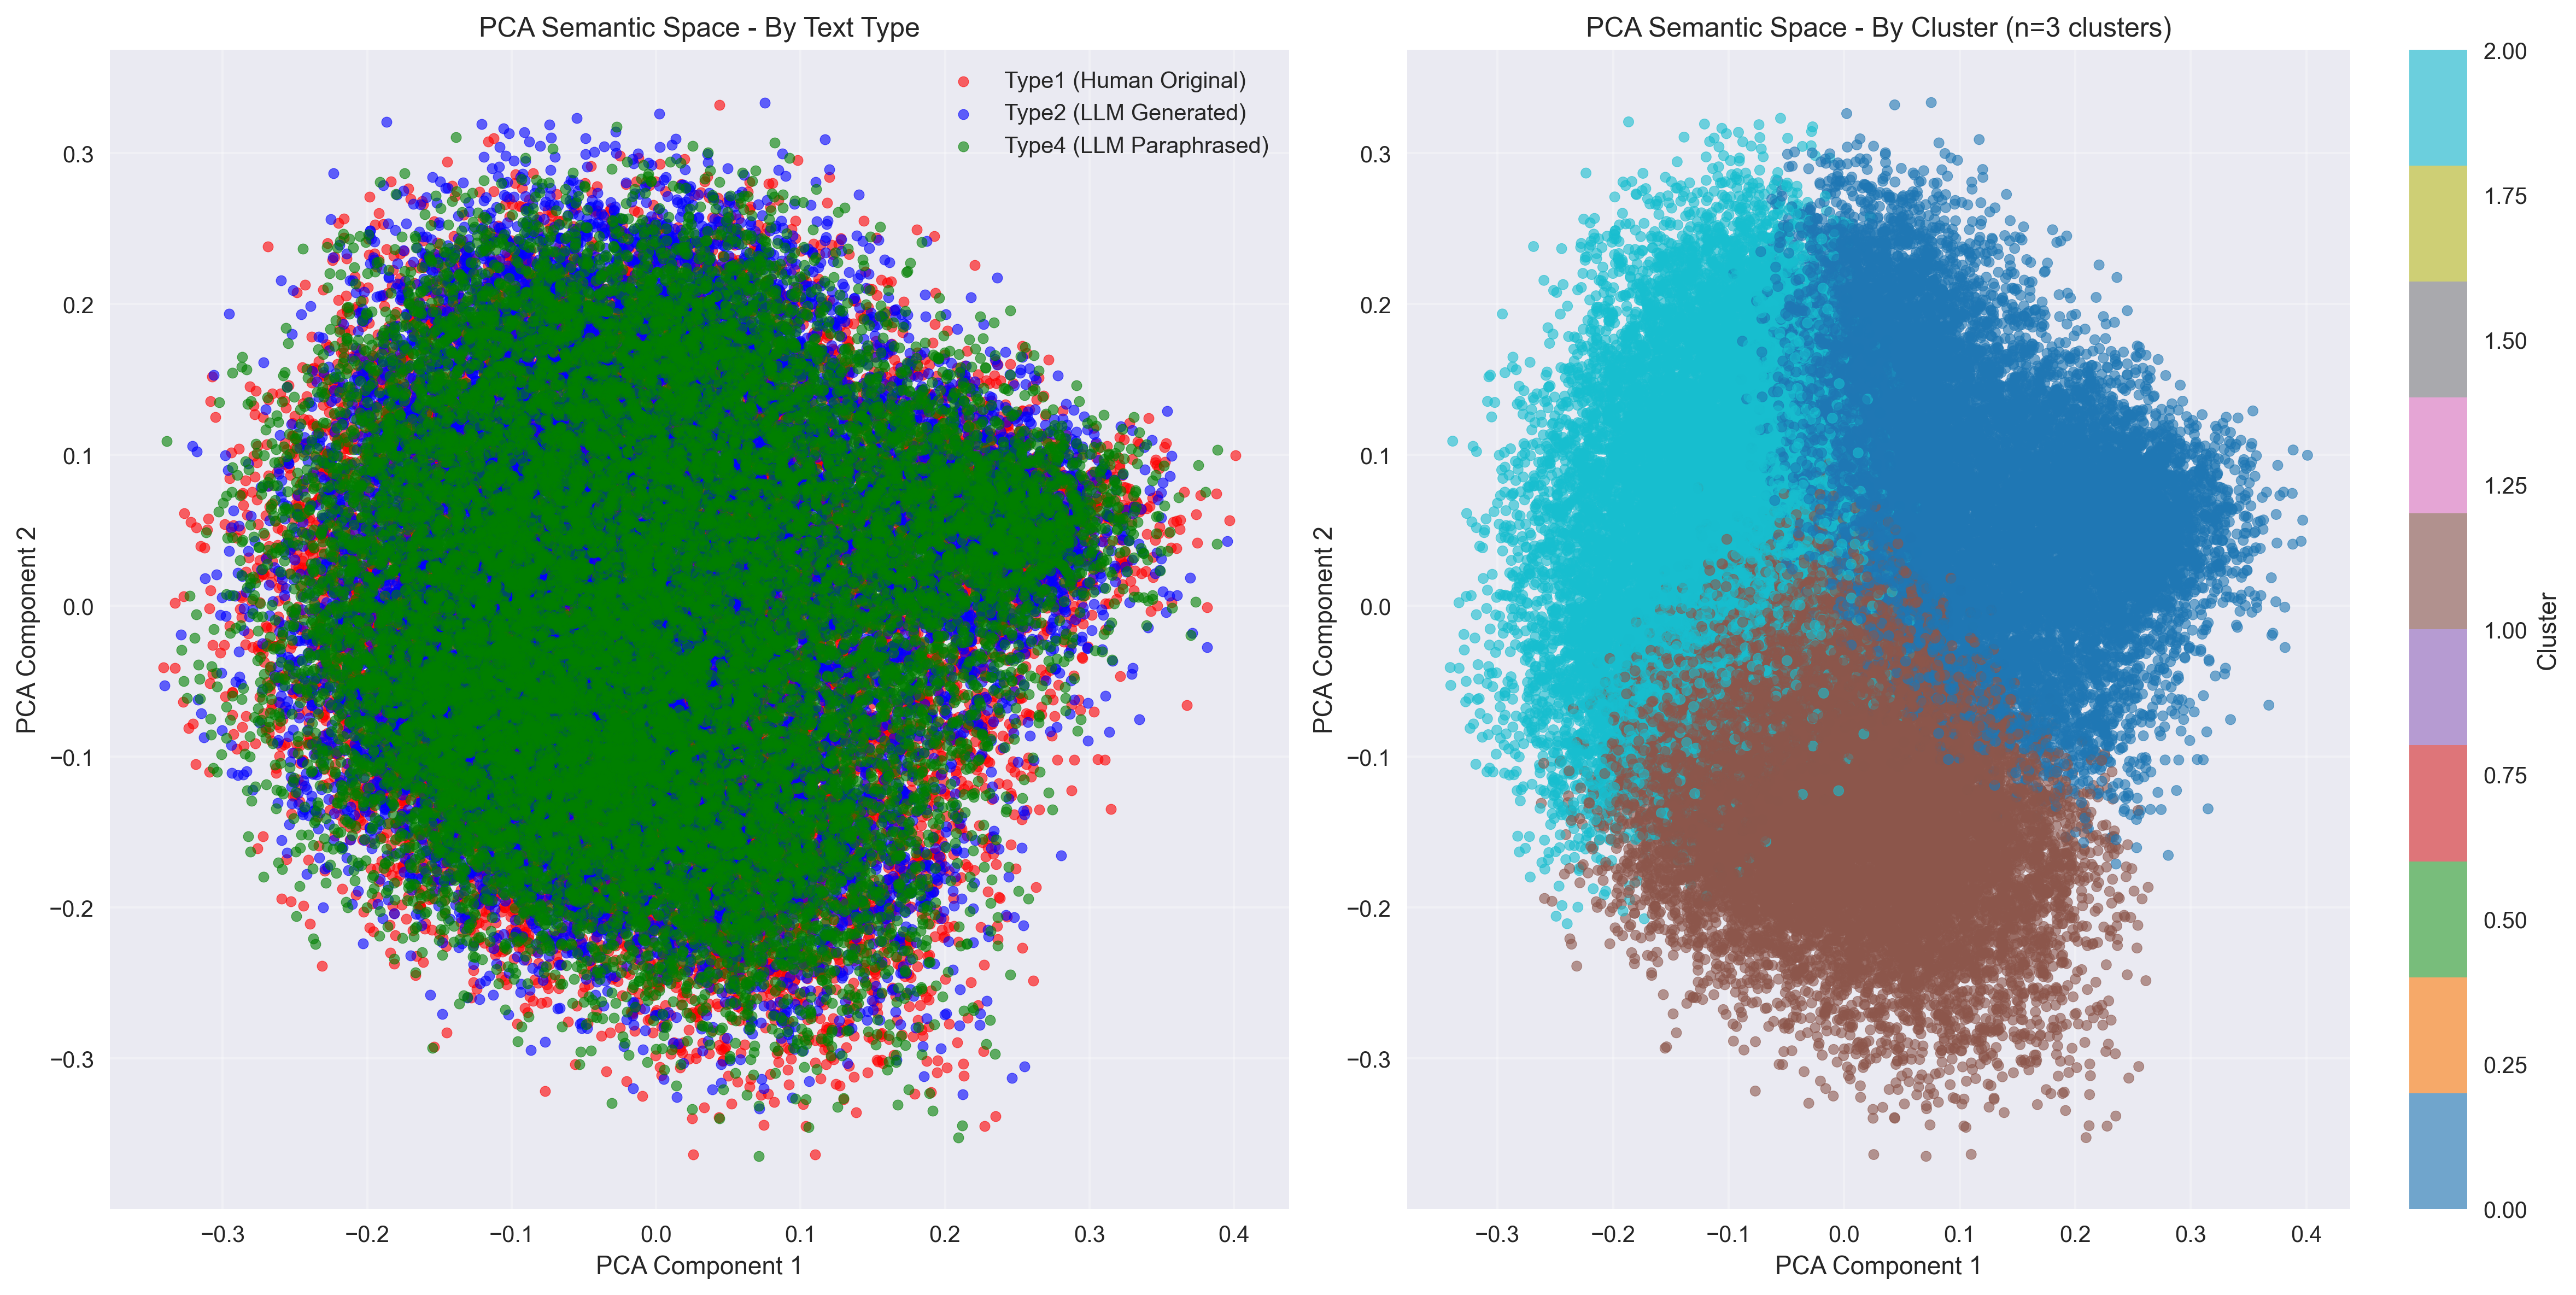
\includegraphics[width=\textwidth]{figures/pca_semantic_space.png}
    \caption{PCA projection of semantic space (left) and K-means clustering results (right, $k=3$). Despite measurable distance differences (Table~\ref{tab:pairwise_distances}), text categories show substantial overlap in 2D projection, indicating that distinguishing information exists in higher dimensions.}
    \label{fig:pca_clustering_appB}
\end{figure}

\noindent\textbf{Distance Metrics}\\
Three complementary distance metrics are computed between embedding pairs to capture different aspects of semantic similarity:
\begin{table}[t]
\centering
\small
\caption{Full Table of Table~\ref{tab:pairwise_distances}, with the addition of Euclidean Distance and Manhattan Distance}
\label{tab:pairwise_distances_appB}
\begin{tabular}{@{}lccc@{}}
\toprule
\textbf{Comparison} & \textbf{Cosine} & \textbf{Eucl.} & \textbf{Manh.} \\
\midrule
Human $\leftrightarrow$ LLM-Gen. & 0.195 & 0.605 & 15.318 \\
Human $\leftrightarrow$ LLM-Para. & \textbf{0.068} & \textbf{0.355} & \textbf{8.991} \\
LLM-Gen. $\leftrightarrow$ LLM-Para. & 0.214 & 0.637 & 16.129 \\
\bottomrule
\end{tabular}
\end{table}
\paragraph{Cosine Similarity}
\begin{equation}
\label{eq:cosine_similarity}
d_{\text{cosine}}(\mathbf{u}, \mathbf{v}) = 1 - \frac{\mathbf{u} \cdot \mathbf{v}}{|\mathbf{u}||\mathbf{v}|} = 1 - \frac{\sum_{i=1}^{n} u_i v_i}{\sqrt{\sum_{i=1}^{n} u_i^2} \sqrt{\sum_{i=1}^{n} v_i^2}}
\end{equation}
where $\mathbf{u}, \mathbf{v} \in \mathbb{R}^n$. Range: $[0, 1]$ where 0 indicates identical direction and 1 indicates orthogonality.

\paragraph{Euclidean Distance}
\begin{equation}
\label{eq:euclidean_distance}
d_{\text{euclidean}}(\mathbf{u}, \mathbf{v}) = \sqrt{\sum_{i=1}^{n} (u_i - v_i)^2} = |\mathbf{u} - \mathbf{v}|_2
\end{equation}

\paragraph{Manhattan Distance}
\begin{equation}
\label{eq:manhattan_distance}
d_{\text{manhattan}}(\mathbf{u}, \mathbf{v}) = \sum_{i=1}^{n} |u_i - v_i| = |\mathbf{u} - \mathbf{v}|_1
\end{equation}

\paragraph{Pairwise Distance Computation}
For each distance metric $d$, average distances between text type pairs are computed:
\begin{align}
\label{eq:pairwise_distance}
D_{H,L}^{(d)} &= \frac{1}{|E_H| \cdot |E_L|} \sum_{e_h \in E_H} \sum_{e_l \in E_L} d(e_h, e_l) \\
D_{H,P}^{(d)} &= \frac{1}{|E_H| \cdot |E_P|} \sum_{e_h \in E_H} \sum_{e_p \in E_P} d(e_h, e_p) \\
D_{L,P}^{(d)} &= \frac{1}{|E_L| \cdot |E_P|} \sum_{e_l \in E_L} \sum_{e_p \in E_P} d(e_l, e_p)
\end{align}
where $H$, $L$, and $P$ denote human-authored, LLM-generated, and paraphrased text, respectively(shown at Table~\ref{tab:pairwise_distances_appB}).

\subsubsection{Semantic Space Exploration}
\label{appB:experiment1_semantic_space}

\begin{figure}[t]
    \centering
    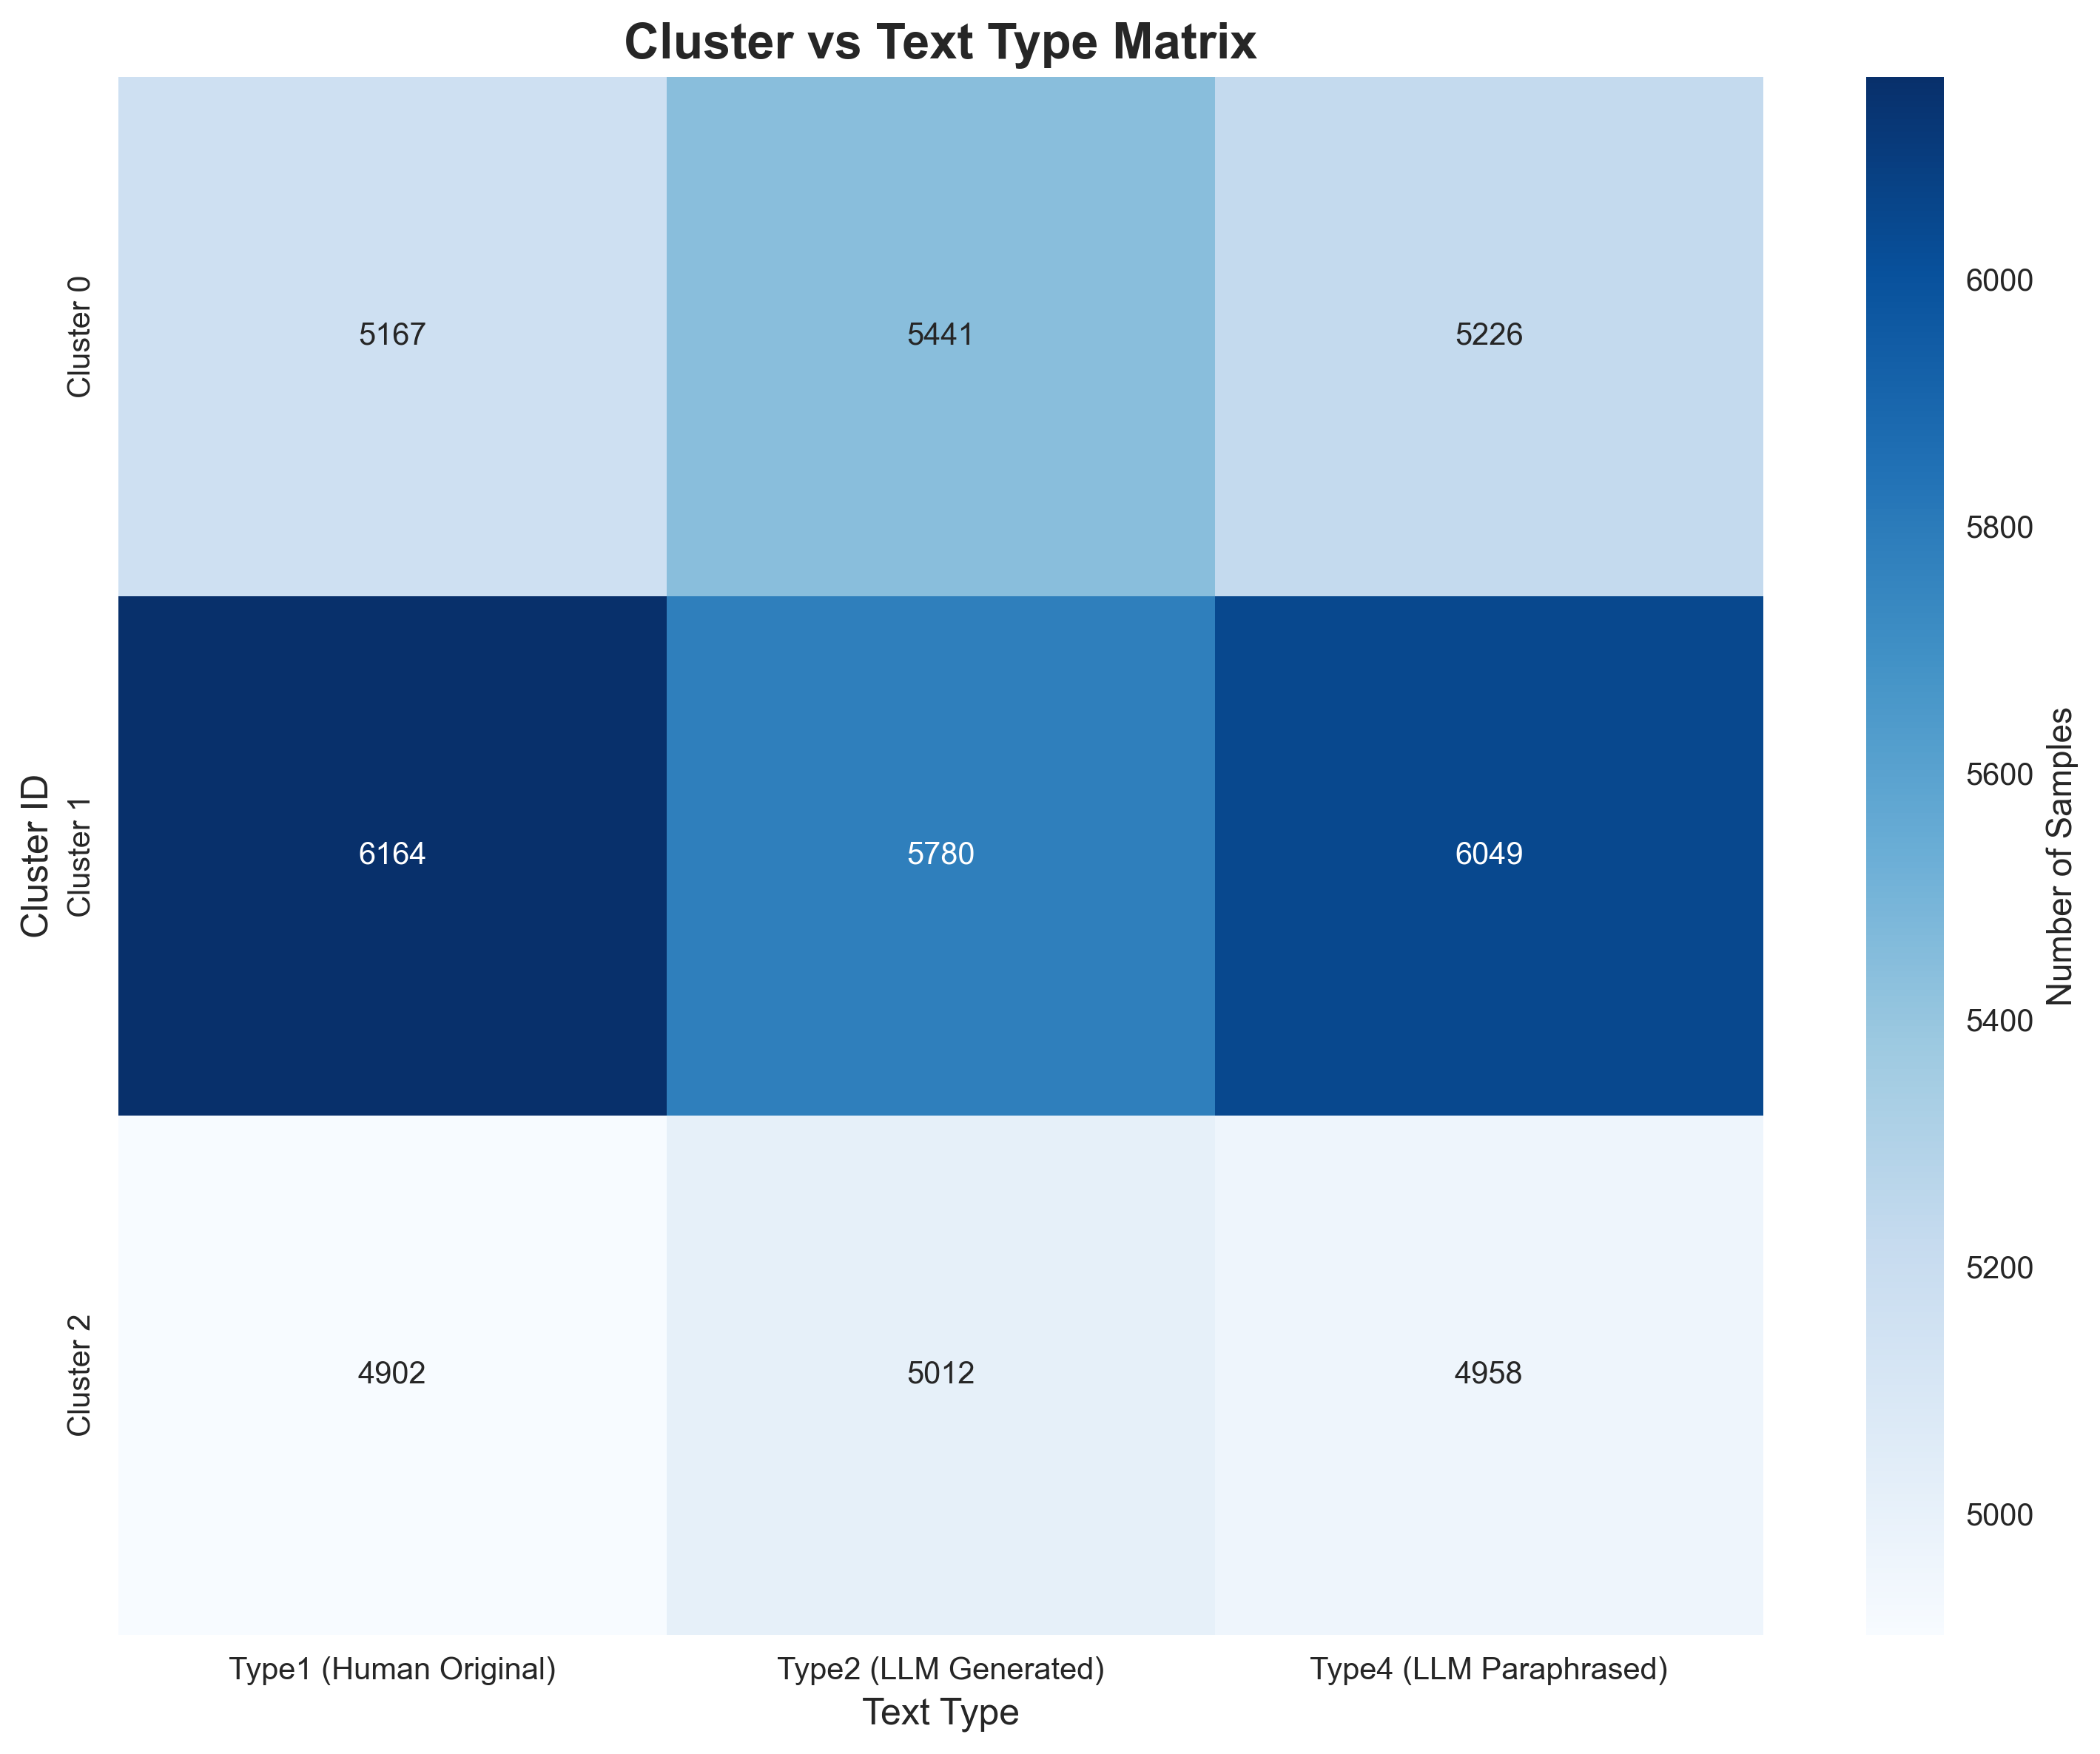
\includegraphics[width=\textwidth]{figures/cluster_type_matrix.png}
    \caption{Clustering label distribution across human-authored, LLM-generated, and LLM-paraphrased text. The matrix reveals that low-dimensional representation space makes it difficult to distinguish between the three text types.}
    \label{fig:cluster_type_matrix}
\end{figure}

\paragraph{Dimensionality Reduction via PCA}
Principal Component Analysis (PCA) is applied to project the high-dimensional BGE-M3 embeddings (1024 dimensions) into 2D visualization space. Figure~\ref{fig:pca_clustering_appB} shows the PCA visualization.

\paragraph{Unsupervised Clustering via KMeans}
K-Means clustering with $k=3$ clusters is applied to the combined embedding space to identify natural semantic groupings. Figure~\ref{fig:pca_clustering_appB} (right) shows the KMeans clustering visualization, and Figure~\ref{fig:cluster_type_matrix} shows the detailed label distribution.

\subsection{Experiment 2: Iterative Paraphrasing in Representation Space}
\label{App:Experiment2}

\subsubsection{Research Objective}
This experiment investigates \textbf{Hypothesis 2}: Iterative paraphrasing makes text become more coherent, deviating from common LLM-generated patterns and moving closer to human-authored texts. Semantic drift is analyzed through multiple iterations of paraphrasing to understand how text evolves in semantic space over successive transformations.

\subsubsection{Data Preparation}
The experiment randomly samples 1000 human-authored texts from the combined dataset (detailed in Appendix~\ref{Appendix_A}).

\subsubsection{Experiment Procedure}

\paragraph{Representation Space Choice}
For each iteration, two complementary representations are extracted:
\begin{enumerate}
    \item \textbf{Hidden States}: Last-layer hidden states from Qwen3-4B-Instruct with mean pooling across sequence length
    \item \textbf{Semantic Embeddings}: BGE-M3 embeddings via Novita AI API for semantic space analysis
\end{enumerate}

\paragraph{Distance Analysis}
Two complementary distance analyses are conducted to examine semantic drift under iterative paraphrasing:

\textbf{Analysis 1: Progressive Semantic Drift.} The distance between consecutive iterations is measured by computing distances between iteration $i$ and iteration $i+1$ for both human-authored and LLM-generated text that have undergone 1--10 paraphrasing iterations. The result table can be found in Table~\ref{tab:iterative_distances}.

\textbf{Analysis 2: Cross-Category Semantic Distance.} Semantic distances are measured between original human-authored text and paraphrased human-authored text (iterations 1--10), as well as between original LLM-generated text and paraphrased human-authored text (iterations 1--10). The result table can be found in Table~\ref{tab:semantic_distances_detailed}.

\begin{table}[t]
\centering
\small
\caption{Cosine similarity: (1) single iteration of paraphrased human-authored text versus 2--10 iterations; (2) single iteration of paraphrased LLM-generated text versus 2--10 iterations, based on BGE-M3 embedding and Qwen3-4B final hidden state. H.\ indicates human-authored text, L.\ indicates LLM-generated text.}
\label{tab:iterative_distances_appB}
\begin{tabular}{@{}p{1cm}lccccc@{}}
\toprule
\multirow{2}{*}{\textbf{Repr.}} & \multirow{2}{*}{\textbf{Type}} & \multicolumn{5}{c}{\textbf{Iteration}} \\
\cmidrule(lr){3-7}
& & \textbf{2} & \textbf{4} & \textbf{6} & \textbf{8} & \textbf{10} \\
\midrule
\multirow{2}{*}{\shortstack[l]{BGE\\Emb.}}
& H & 0.048 & 0.072 & 0.083 & 0.092 & 0.100 \\
& L & 0.047 & 0.068 & 0.077 & 0.087 & 0.091 \\
\midrule
\multirow{2}{*}{\shortstack[l]{Hid.\\Stat.}}
& H & 0.012 & 0.022 & 0.015 & 0.017 & 0.019 \\
& L & 0.011 & 0.014 & 0.015 & 0.017 & 0.018 \\
\bottomrule
\end{tabular}
\end{table}

\begin{table}[t]
\centering
\small
\caption{Semantic distance between two text types: (1) human-authored text versus 1--10 iterations of paraphrased human-authored text; (2) LLM-generated text versus 1--10 iterations of paraphrased human-authored text.}
\label{tab:semantic_distances_detailed}
\begin{tabular}{@{}llcc@{}}
\toprule
\multirow{2}{*}{\textbf{Text Type}} & \multirow{2}{*}{\textbf{Iter.}} & \textbf{Cosine} & \textbf{Euclidean} \\
& & \textbf{Distance} & \textbf{Distance} \\
\midrule
\multirow{10}{*}{\shortstack[l]{Human-\\Authored}}
& 1 & 0.064 & 0.342 \\
& 2 & 0.085 & 0.394 \\
& 3 & 0.099 & 0.426 \\
& 4 & 0.107 & 0.443 \\
& 5 & 0.118 & 0.465 \\
& 6 & 0.122 & 0.472 \\
& 7 & 0.125 & 0.478 \\
& 8 & 0.128 & 0.484 \\
& 9 & 0.129 & 0.486 \\
& 10 & 0.134 & 0.494 \\
\midrule
\multirow{10}{*}{\shortstack[l]{LLM-\\Generated}}
& 1 & 0.700 & 1.182 \\
& 2 & 0.698 & 1.180 \\
& 3 & 0.696 & 1.179 \\
& 4 & 0.697 & 1.180 \\
& 5 & 0.696 & 1.179 \\
& 6 & 0.697 & 1.179 \\
& 7 & 0.697 & 1.180 \\
& 8 & 0.699 & 1.181 \\
& 9 & 0.697 & 1.179 \\
& 10 & 0.698 & 1.180 \\
\bottomrule
\end{tabular}
\end{table}

For both analyses, three complementary distance metrics are employed to capture different aspects of semantic dissimilarity: cosine similarity, Euclidean distance, and Manhattan distance (see Equations~\ref{eq:cosine_similarity},~\ref{eq:euclidean_distance}, and~\ref{eq:manhattan_distance}).

Analysis 1 uses centroid-based distance to measure population-level drift. For each iteration $i$ and text type $t$, population centroids are computed:
\begin{equation}
\mathbf{c}_{i,t} = \frac{1}{N} \sum_{j=1}^{N} \mathbf{e}_{i,t,j}
\end{equation}
where $\mathbf{e}_{i,t,j}$ represents the embedding of sample $j$ at iteration $i$ for text type $t$. Sequential distance analysis then tracks semantic drift between consecutive iterations:
\begin{equation}
\Delta d_{i \rightarrow i+1} = d(\mathbf{c}_{i,t}, \mathbf{c}_{i+1,t})
\end{equation}

Analysis 2 employs the pairwise distance calculation described in Equation~\ref{eq:pairwise_distance}, measuring distances between the reference texts (human-authored original and LLM-generated original) and iteratively paraphrased human-authored text at each iteration level.

\paragraph{PCA Trajectory Analysis}

\begin{figure}[t]
    \centering
    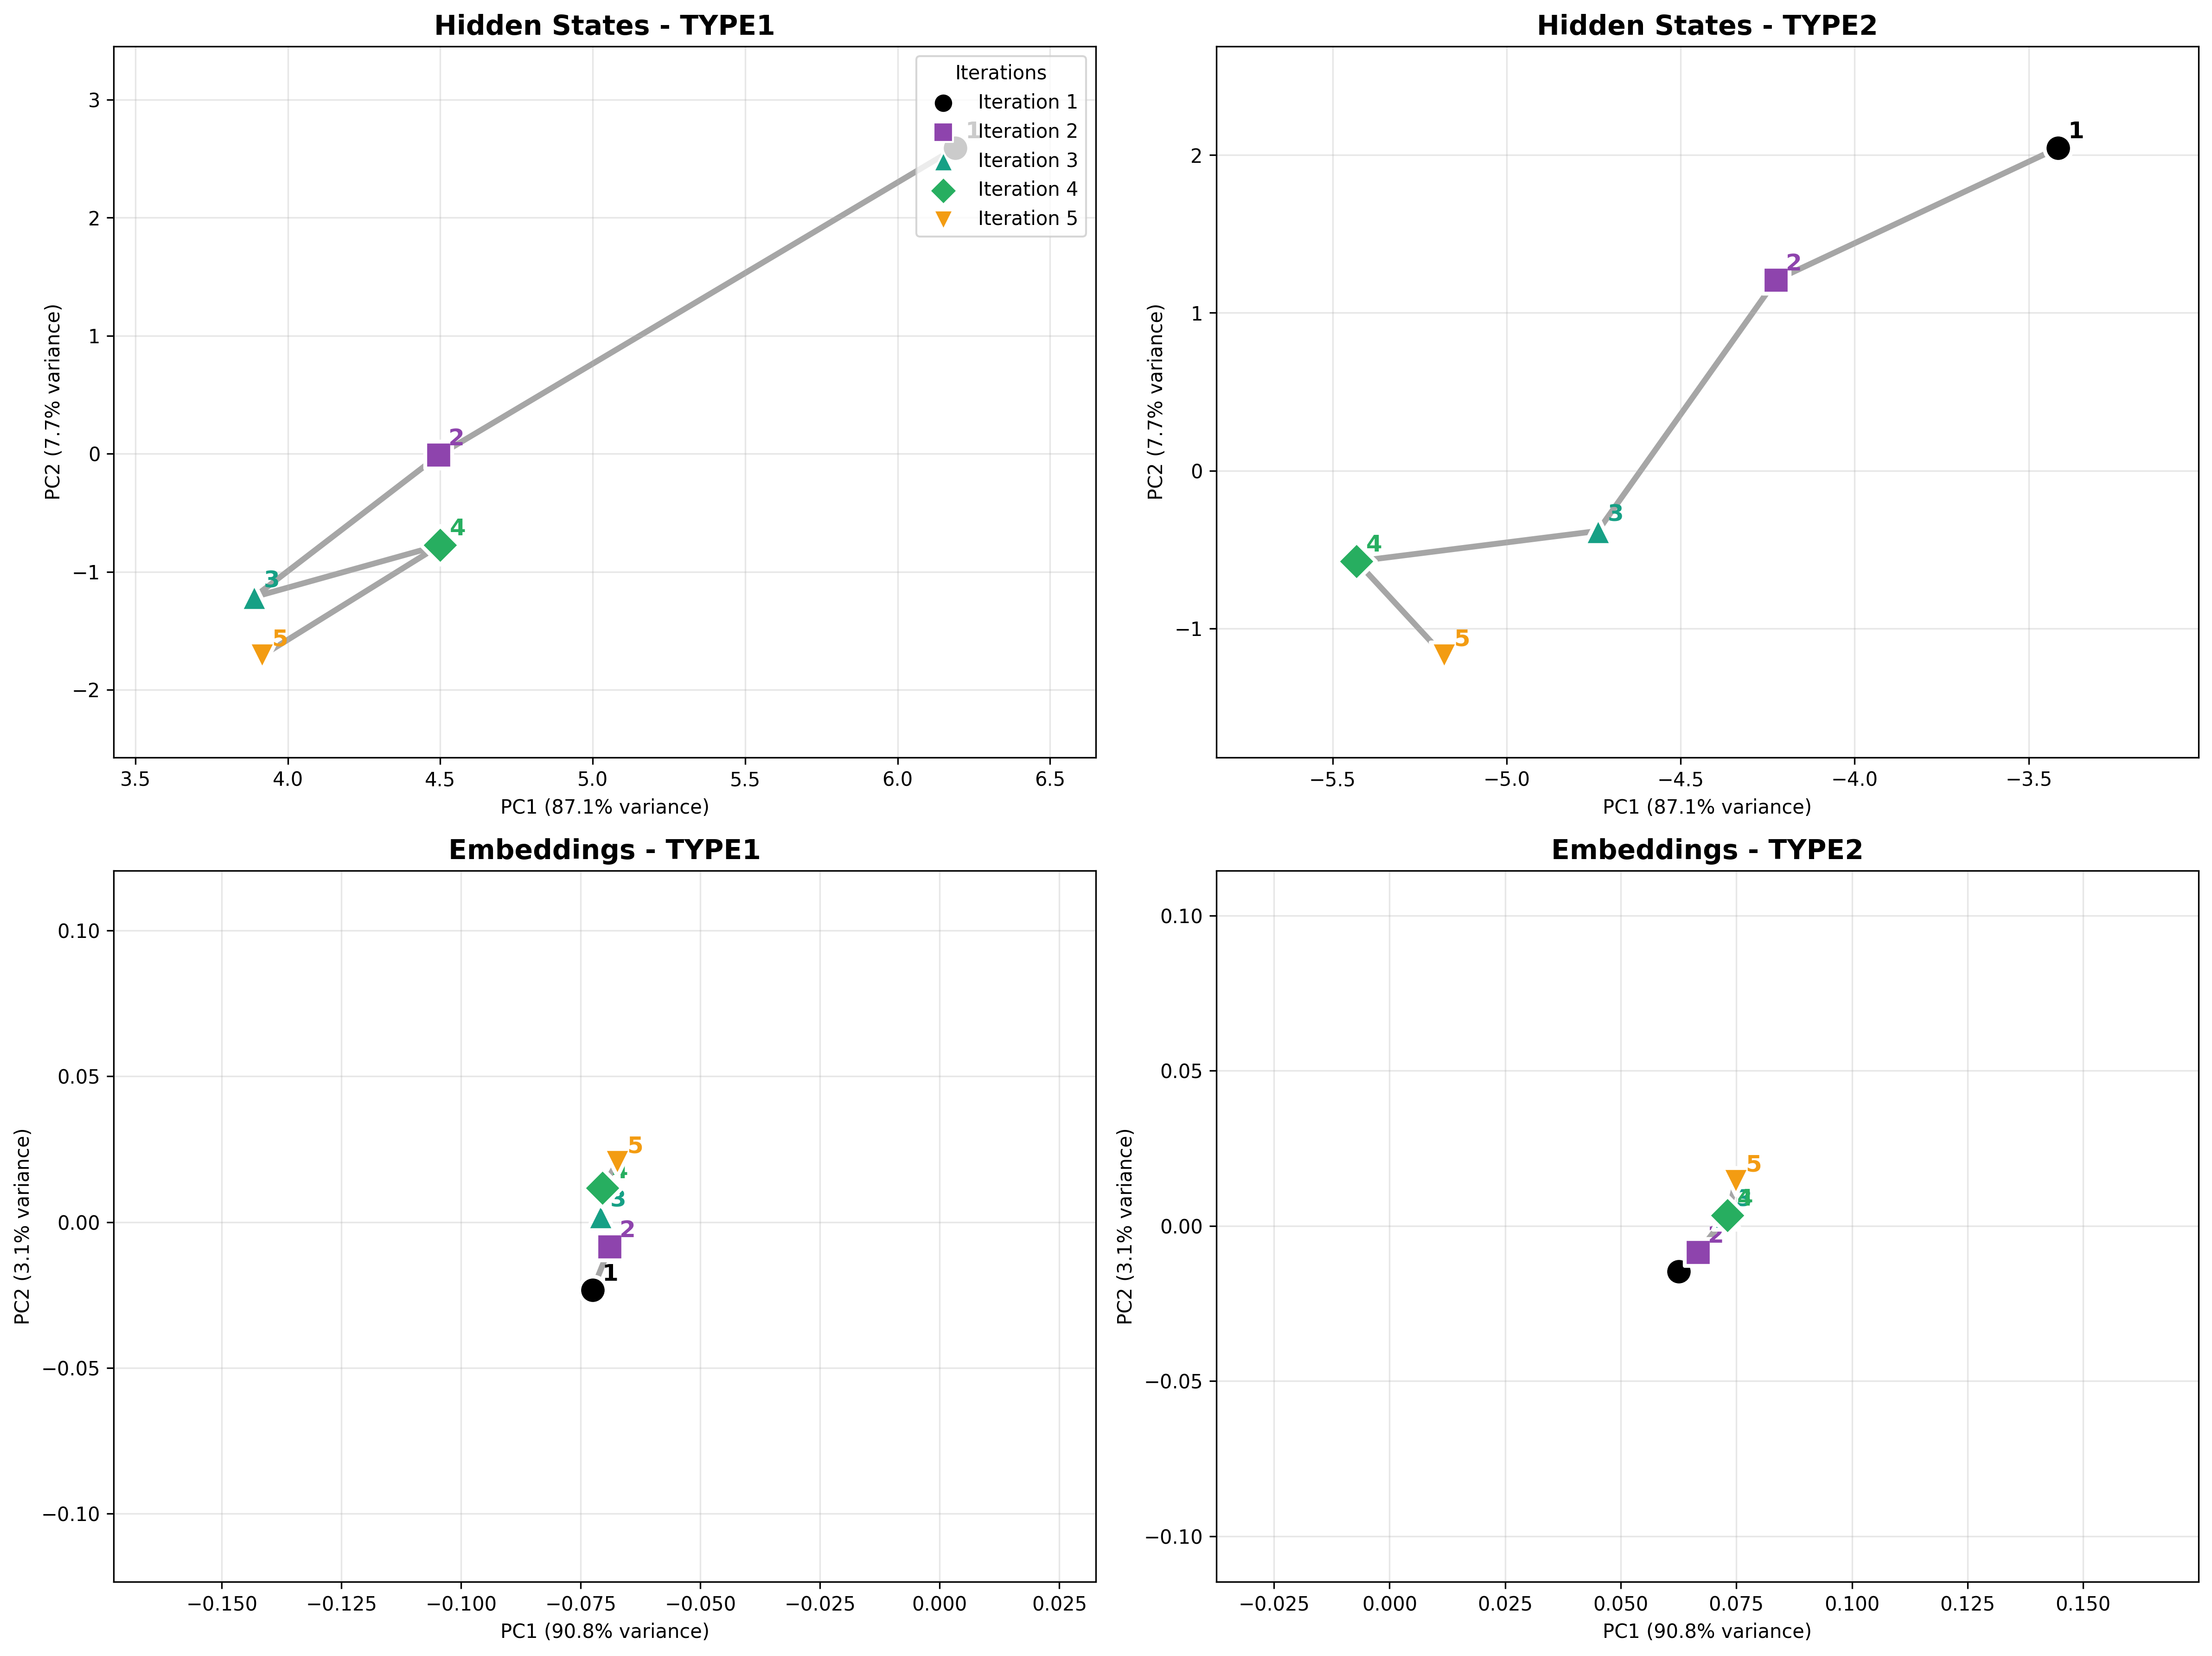
\includegraphics[width=\textwidth]{figures/centroid_trajectories_5itr.png}
    \caption{The 5-iteration centroid trajectories under PCA ($n=2$). Top: Hidden state space (left: human-origin, right: LLM-origin). Bottom: Embedding space.}
    \label{fig:trajectories_5itr}
\end{figure}

\begin{figure}[t]
    \centering
    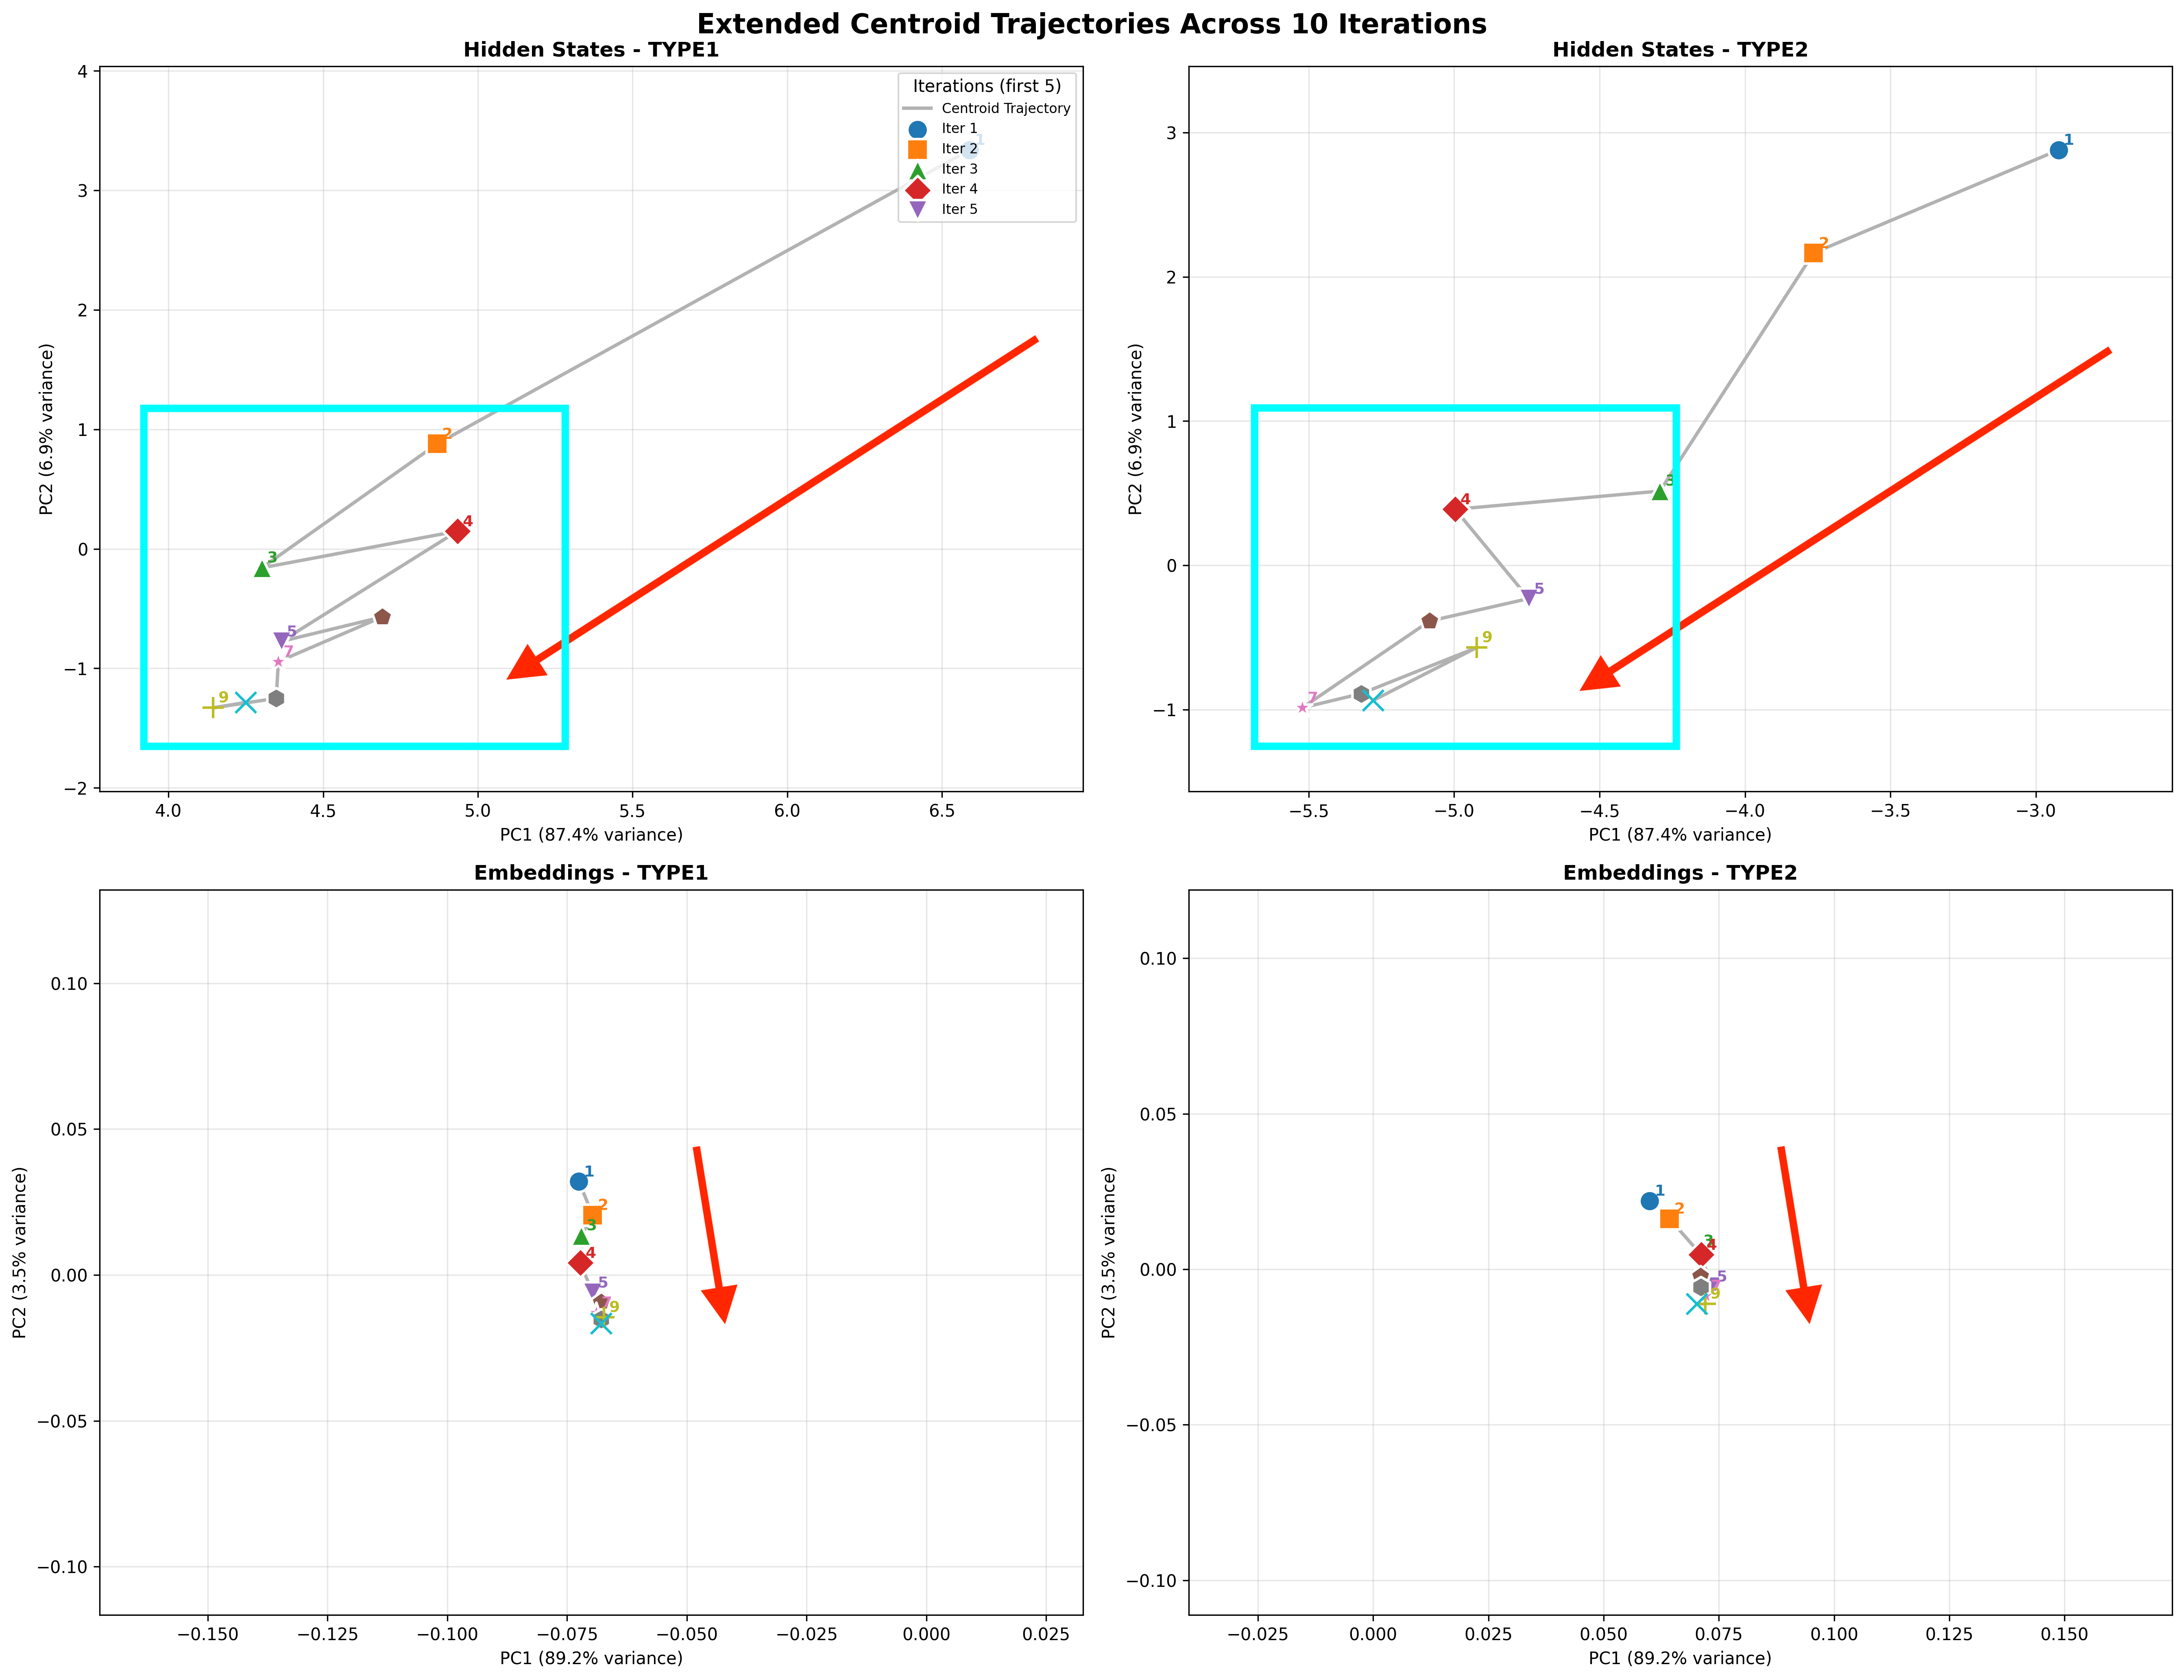
\includegraphics[width=\textwidth]{figures/centroid_trajectories_10iter.png}
    \caption{Extended 10-iteration centroid trajectories showing semantic drift patterns. Top: Hidden state space (left: human-origin, right: LLM-origin). Bottom: Embedding space. Both origins move in parallel directions, with trajectories converging toward overlapping regions in later iterations.}
    \label{fig:trajectories_10itr}
\end{figure}

PCA is applied to project high-dimensional embeddings into 2D visualization space. This trajectory analysis tracks how text representations evolve through successive paraphrasing iterations.

A 5-iteration analysis was initially conducted to identify semantic drift patterns. However, the resulting trajectories did not reveal sufficiently clear patterns to draw robust conclusions about long-term semantic behavior (Figure~\ref{fig:trajectories_5itr}). Consequently, the analysis was extended to 10 iterations, which provided more definitive evidence of semantic drift trajectories and convergence patterns.

The PCA trajectory analysis follows the procedure outlined in Algorithm~\ref{alg:pca_trajectory}:

\begin{algorithm}[H]
\caption{PCA Trajectory Analysis}
\label{alg:pca_trajectory}
\begin{algorithmic}[1]
\STATE Collect all embeddings across iterations: $E = \{\mathbf{e}_{i,t,j} : i \in [1,N_{iter}], t \in \{\text{type1}, \text{type2}\}, j \in [1,N_{samples}]\}$
\STATE Standardize features: $\tilde{E} = \text{StandardScaler}(E)$
\STATE Apply PCA: $E_{\text{PCA}} = \text{PCA}_{n=2}(\tilde{E})$
\STATE Compute iteration centroids in PCA space: $\mathbf{c}_{i,t}^{\text{PCA}} = \frac{1}{N} \sum_{j=1}^{N} \mathbf{e}_{i,t,j}^{\text{PCA}}$
\STATE Track centroid trajectories: $\mathcal{T}_t = \{\mathbf{c}_{i,t}^{\text{PCA}} : i \in [1,N_{iter}]\}$
\end{algorithmic}
\end{algorithm}

To quantify the magnitude of semantic drift, the total Euclidean displacement of centroids across iterations is computed:
\begin{equation}
\text{Total Drift}_t = \sum_{i=1}^{N_{iter}-1} ||\mathbf{c}_{i+1,t}^{\text{PCA}} - \mathbf{c}_{i,t}^{\text{PCA}}||_2
\end{equation}

Figure~\ref{fig:trajectories_10itr} visualizes the resulting trajectories in PCA space, where each point represents the centroid of all samples at a given iteration, and connecting lines trace the semantic evolution path.

\paragraph{Detailed Interpretation of Figure~\ref{fig:trajectories_10itr}.}
The 10-iteration centroid trajectories reveal four key patterns:

\begin{enumerate}[nosep]
    \item \textbf{Universal directional drift (embedding space, bottom row).} In BGE-M3 embedding space, centroids from both human-origin and LLM-origin texts move consistently in similar directions across iterations. The trajectories do not oscillate but show a steady, gradual displacement---consistent with Table~\ref{tab:semantic_distances}, which shows monotonically increasing cosine similarity from the human-authored reference. This uniform drift across origins suggests that the paraphrasing operation itself (regardless of source) pushes texts in a common direction in semantic embedding space.

    \item \textbf{Oscillatory behavior in hidden states (top row).} Hidden-state centroids show a different pattern: an initial displacement in the first few iterations followed by oscillations around a fixed region rather than continued drift. This is consistent with Table~\ref{tab:iterative_distances}, where inter-iteration hidden-state distances plateau or fluctuate (values 0.012--0.022) without accumulating. The oscillatory behavior suggests generation-level features are not systematically altered by paraphrasing---the LLM paraphraser reorganizes surface text but does not consistently shift the statistical generation signature.

    \item \textbf{Trajectory convergence toward overlapping regions.} By iteration 8--10, the PCA centroids of human-origin and LLM-origin trajectories approach overlapping regions in both hidden-state and embedding spaces. This convergence in low-dimensional PCA space motivates the design of the benchmark tasks: if trajectories from different origins visually converge, distinguishing source origin (Task 3) or iteration depth (Task 4) becomes increasingly difficult for detectors relying on embedding-space signals.

    \item \textbf{Asymmetry between origins.} While trajectories converge, the starting positions differ substantially. Human-origin centroids begin in the upper portion of PCA space; LLM-origin centroids begin in a distinct cluster. The convergence therefore requires traversal of the full distance between these starting regions over 10 iterations---a distance not fully closed in 1--3 iterations, explaining why Task 5 (human original vs.\ 3-iteration laundered AI) remains tractable: at 3 iterations, the LLM-origin trajectory has not yet fully overlapped with the human-origin region.
\end{enumerate}

\section{Detailed Methodology}
\label{Appendix_C}

\subsection{Dataset Preparation}
The benchmark builds upon the human-authored sentences (Type 1) and human paraphrases (Type 3) from three established datasets: MRPC, HLPC, and PAWS. The detailed preprocessing pipeline, including deduplication and quality control procedures, is described in Appendix~\ref{Appendix_A}. This foundation provides 16,233 unique human-authored sentences and human-paraphrased human texts, from which the remaining text types (Type 2, 4, 5) are systematically generated using the pipeline described in Appendix~\ref{appC:data_generation}.

\subsection{Text Type Taxonomy}
\label{appC:taxonomy_definition}
A five-category taxonomy is established to systematically analyze different text generation and paraphrasing patterns:

\begin{itemize}
    \item \textbf{Type 1}: Human original text --- authentic human-authored sentences
    \item \textbf{Type 2}: LLM-generated text --- synthetically generated content maintaining semantic equivalence to Type 1 (generated by sentence completion method)
    \item \textbf{Type 3}: Human-paraphrased human original text --- human-authored paraphrases of Type 1 sentences
    \item \textbf{Type 4}: LLM-paraphrased human original text --- machine-generated paraphrases of Type 1 sentences
    \item \textbf{Type 5}: LLM-iteratively-paraphrased LLM-generated text --- machine-generated paraphrases of Type 2 sentences with multiple iteration levels
\end{itemize}

\subsection{Data Generation Pipeline}
\label{appC:data_generation}

\subsubsection{Technical Architecture}
The data generation system employs a modular, configuration-driven architecture with model selection optimized for each text type's specific requirements. The use of multiple models for paraphrasing (Type 4 and 5) is a deliberate choice to create a diverse dataset that is not biased toward the stylistic quirks of a single paraphraser.

The pipeline implements three sequential generation modules:
\begin{enumerate}
    \item \textbf{Type 2 Generation Module}: Sentence completion-based text synthesis using \textbf{Google Gemini-2.5-Pro}
    \item \textbf{Type 4 Generation Module}: Multiple-model paraphrasing combining DIPPER paraphraser \cite{krishna2023paraphrasingevadesdetectorsaigenerated}, Gemini-2.5-Pro with prompt-based instructions, and LLaMA-3-8B paraphrase fine-tuned models \cite{mradermacher2024llama31paraphrase}
    \item \textbf{Type 5 Generation Module}: Iterative paraphrasing using the same multi-model approach as Type 4
\end{enumerate}

\subsubsection{Type 2 Generation: Sentence Completion Method}

A \textbf{sentence completion approach} is implemented for Type 2 text generation, designed to produce text that is contextually grounded in the original human sentence while allowing for natural, unconstrained continuation. The process involves:

\begin{enumerate}
    \item \textbf{Keyword Extraction}: Using SpaCy's named entity recognition and dependency parsing to identify salient keywords from Type 1 sentences
    \item \textbf{Prefix Extraction}: Extracting the first 20\% of tokens from the original sentence as contextual seed
    \item \textbf{Length Constraints}: Computing target length parameters with $\pm$20\% tolerance
\end{enumerate}

\noindent\textbf{Generation Prompt Template}
\begin{quote}
\small
\texttt{Continue this text naturally and coherently:}

\texttt{``\{sentence\_prefix\}''}

\texttt{Requirements:}
\begin{itemize}[nosep,leftmargin=1em]
    \item \texttt{Target length: \textasciitilde\{target\_length\} characters total}
    \item \texttt{Maximum length: \{max\_length\} characters}
    \item \texttt{Keywords to include: \{keywords\}}
    \item \texttt{Write in a natural, fluent style}
\end{itemize}

\texttt{Return ONLY the completed text with no labels, quotes, explanations, or alternatives.}

\texttt{Completion:}
\end{quote}

\subsubsection{Type 4 Generation: Direct Paraphrasing}
Type 4 generation employs \textbf{prompt-based paraphrasing} using carefully engineered instructions, prioritizing semantic preservation while encouraging significant lexical and syntactic variation.

\noindent\textbf{Paraphrasing Prompt Template}
\begin{quote}
\small
\texttt{Please paraphrase the following text while maintaining its original meaning:}

\texttt{\{text\}}

\texttt{Paraphrased text:}
\end{quote}

\subsubsection{Type 5 Generation: Iterative Paraphrasing}
The Type 5 module implements \textbf{multi-iteration paraphrasing} of Type 2 texts. Two levels are supported: 1 and 3 iterations, where each iteration applies the paraphrasing prompt to the output of the previous one.

\textbf{Iteration Control Mechanisms}:
\begin{itemize}
    \item \textbf{Temperature Scaling}: Base temperature (0.8) increases by 0.1--0.15 per iteration level to enhance diversity
    \item \textbf{Convergence Detection}: Automatic termination when consecutive iterations achieve $>$95\% similarity
    \item \textbf{Length Tolerance}: Expanded to $\pm$40\% to accommodate cumulative variation across iterations
\end{itemize}

\subsection{Data Quality Assessment}
\label{appC:data_quality}

Three complementary quality metrics are employed: \textbf{Jaccard similarity}, \textbf{perplexity}, and \textbf{self-BLEU} scores.

\textbf{Jaccard Similarity Analysis}: The inter-type similarity matrix reveals expected semantic relationships across text types. Human original text (Type 1) demonstrates highest similarity with human paraphrases (Type 3, Jaccard = 0.798), confirming semantic preservation in human paraphrasing. Notably, iterative paraphrasing exhibits controlled diversity: Type 5 first-iteration maintains reasonable similarity with its source (0.469 with Type 2), while third-iteration paraphrasing shows increased lexical divergence (0.423 with Type 2).

\begin{figure}[htbp]
    \centering
    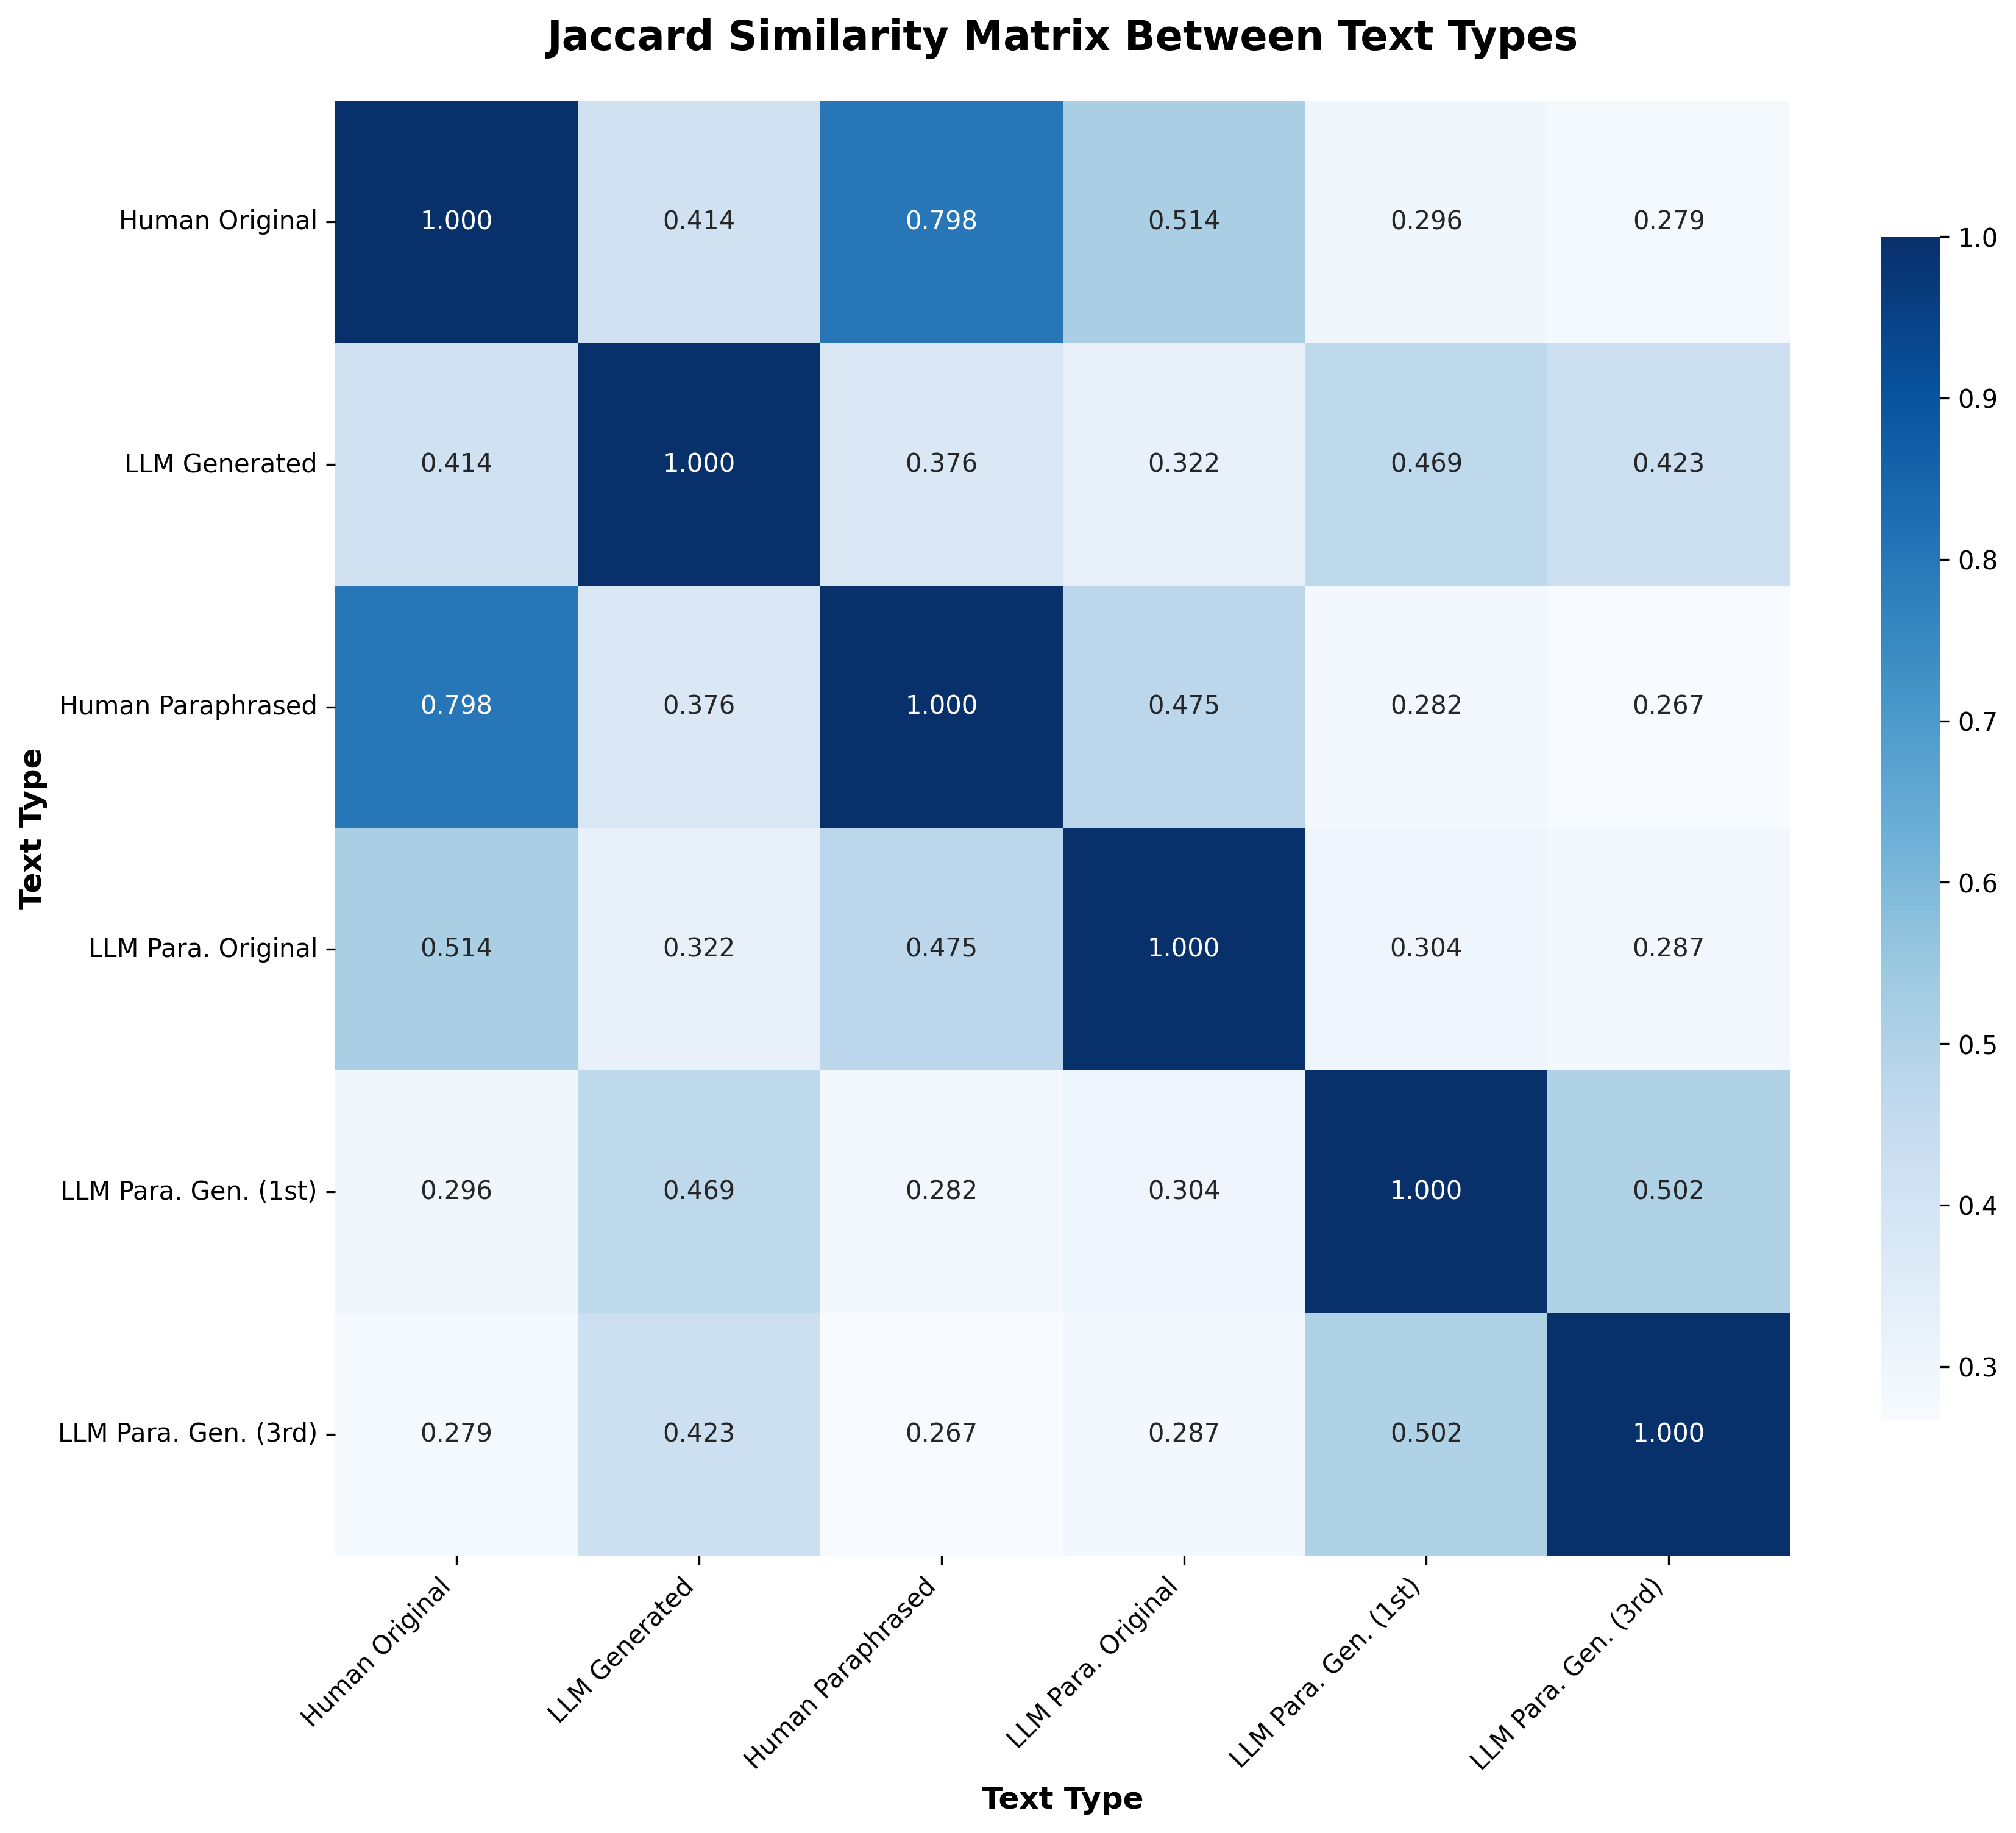
\includegraphics[width=0.5\textwidth]{figures/similarity_heatmap.png}
    \caption{Jaccard similarity matrix between different text types.}
    \label{fig:jaccard_similarity}
\end{figure}

\textbf{Perplexity Evaluation}: Text predictability is assessed using perplexity scores computed with GPT-2-XL and LLaMA-2-7B as reference models. The quality metrics reveal consistent patterns across both evaluation models (Table~\ref{tab:quality_metrics}). LLM-generated text (Type 2) exhibits the lowest perplexity scores (GPT-2-XL: 77.84, LLaMA-2-7B: 42.61), while human original and paraphrased texts consistently demonstrate higher perplexity scores, suggesting greater linguistic variability.

\begin{table}[htbp]
\centering
\caption{Quality metrics across text types.}
\label{tab:quality_metrics}
\footnotesize
\begin{tabular}{lccc}
\hline
\textbf{Text Type} & \textbf{PPL-G2X} & \textbf{PPL-L7B} & \textbf{sBLEU} \\
\hline
Type 1 & 106.78 & 49.57 & 0.268 \\
Type 2 & 77.84 & 42.61 & 0.242 \\
Type 3 & 107.47 & 49.45 & 0.275 \\
Type 4 & 85.90 & 39.63 & 0.196 \\
Type 5-1st & 99.63 & 47.29 & 0.179 \\
Type 5-3rd & 109.32 & 50.23 & 0.170 \\
\hline
\textbf{Average} & \textbf{97.82} & \textbf{46.46} & \textbf{0.222} \\
\hline
\end{tabular}
\end{table}

\textbf{Self-BLEU Assessment}: Self-BLEU scores (Table~\ref{tab:quality_metrics}) demonstrate appropriate diversity levels across all text types, with iterative paraphrasing achieving maximum diversity (Type 5-3rd: 0.170).

\begin{table}[htbp]
\centering
\caption{Quality metrics comparison between PADBen and RAID datasets (average values).}
\label{tab:dataset_comparison}
\begin{tabular}{lccc}
\hline
\textbf{Dataset} & \textbf{Self-BLEU} & \textbf{PPL-G2X} & \textbf{PPL-L7B} \\
\hline
PADBen & 0.222 & 97.82 & 46.46 \\
RAID & 13.7 & 23.8 & 6.6 \\
\hline
\end{tabular}
\end{table}

\textbf{Comparison with RAID}: PADBen exhibits substantially lower self-BLEU scores (0.222 vs 13.7), indicating approximately 62$\times$ higher intra-type diversity. Using GPT-2-XL, PADBen achieves 4.1$\times$ higher perplexity scores (97.82 vs 23.8), while LLaMA-2-7B evaluation shows a 7.0$\times$ difference (46.46 vs 6.61).

\subsection{Dataset Statistics}
The final dataset comprises \textbf{16,232 sentence groups} across three source datasets, each containing all five text types.

\subsection{Detailed Task Introduction}
\label{appC:task_intro}

\subsubsection{Task 1: Paraphrase Source Attribution}
\textbf{Objective}: Evaluate detectors' ability to distinguish between human and machine paraphrasing without access to original source text.

\textbf{Data Configuration}: Utilize Type 3 (human-paraphrased) and Type 4 (LLM-paraphrased) texts. Human paraphrases are labeled as 0, LLM-generated paraphrases as 1.

\textbf{Detection Challenge}: Without reference to original text, detectors must rely solely on intrinsic linguistic markers to differentiate human and machine paraphrasing strategies.

\subsubsection{Task 2: General Text Authorship Detection}
\textbf{Objective}: Assess baseline detection performance distinguishing original human-authored text from LLM-generated content.

\textbf{Data Configuration}: Utilize Type 1 (human original) and Type 2 (LLM-generated) texts. Human-authored content is labeled as 0, LLM-generated text as 1.

\subsubsection{Task 3: AI Text Laundering Detection}
\textbf{Objective}: Evaluate detectors' resilience against AI text laundering through paraphrasing attacks.

\textbf{Data Configuration}: Utilize Type 4 (LLM-paraphrased human text) and Type 5-1st (single-iteration LLM-paraphrased LLM text). LLM-paraphrased human content is labeled as 0, laundered AI text as 1.

\textbf{Detection Challenge}: Both texts have undergone identical machine transformation, requiring determination of which originated from human versus LLM sources before paraphrasing.

\subsubsection{Task 4: Iterative Paraphrase Depth Detection}
\textbf{Objective}: Assess detector ability to distinguish between shallow and deep iterative paraphrasing attacks.

\textbf{Data Configuration}: Utilize Type 5-1st (single-iteration) and Type 5-3rd (triple-iteration) paraphrased LLM text. Shallow paraphrasing (1 iteration) is labeled as 0, deep paraphrasing (3 iterations) as 1.

\subsubsection{Task 5: Paraphrase Attack Detection}
\textbf{Objective}: Evaluate detector resilience in the ultimate end-to-end evasion scenario.

\textbf{Data Configuration}: Utilize Type 1 (human original) and Type 5-3rd (triple-iteration LLM-paraphrased LLM text). Human text is labeled as 0, deeply laundered AI text as 1.

\textbf{Detection Challenge}: This is the benchmark's final stress test, requiring detectors to identify highly subtle, persistent machine-generation artifacts that have survived multiple layers of transformation.

\section{Detailed Task Data Setup}
\label{appD:evaluation_setup}

\begin{algorithm}[H]
\caption{Single-Sentence Exhaustive Method}
\begin{algorithmic}[1]
\label{algo:exhaustive_method}
\STATE \textbf{Input:} Dataset $D$ with $n$ samples, Task specification $(T_A, T_B)$
\STATE \textbf{Initialize:} $samples \leftarrow \emptyset$
\FOR{each sample $s_i \in D$}
    \STATE Extract text $text_A \leftarrow s_i[T_A]$
    \STATE Extract text $text_B \leftarrow s_i[T_B]$
    \STATE Create sample: $(idx=2i, sentence=text_A, label=0)$
    \STATE Create sample: $(idx=2i+1, sentence=text_B, label=1)$
\ENDFOR
\STATE Shuffle sample indices randomly
\STATE \textbf{Output:} Dataset of size $2n$ with balanced 50-50 label distribution
\end{algorithmic}
\end{algorithm}
\begin{figure}[t]
    \centering
    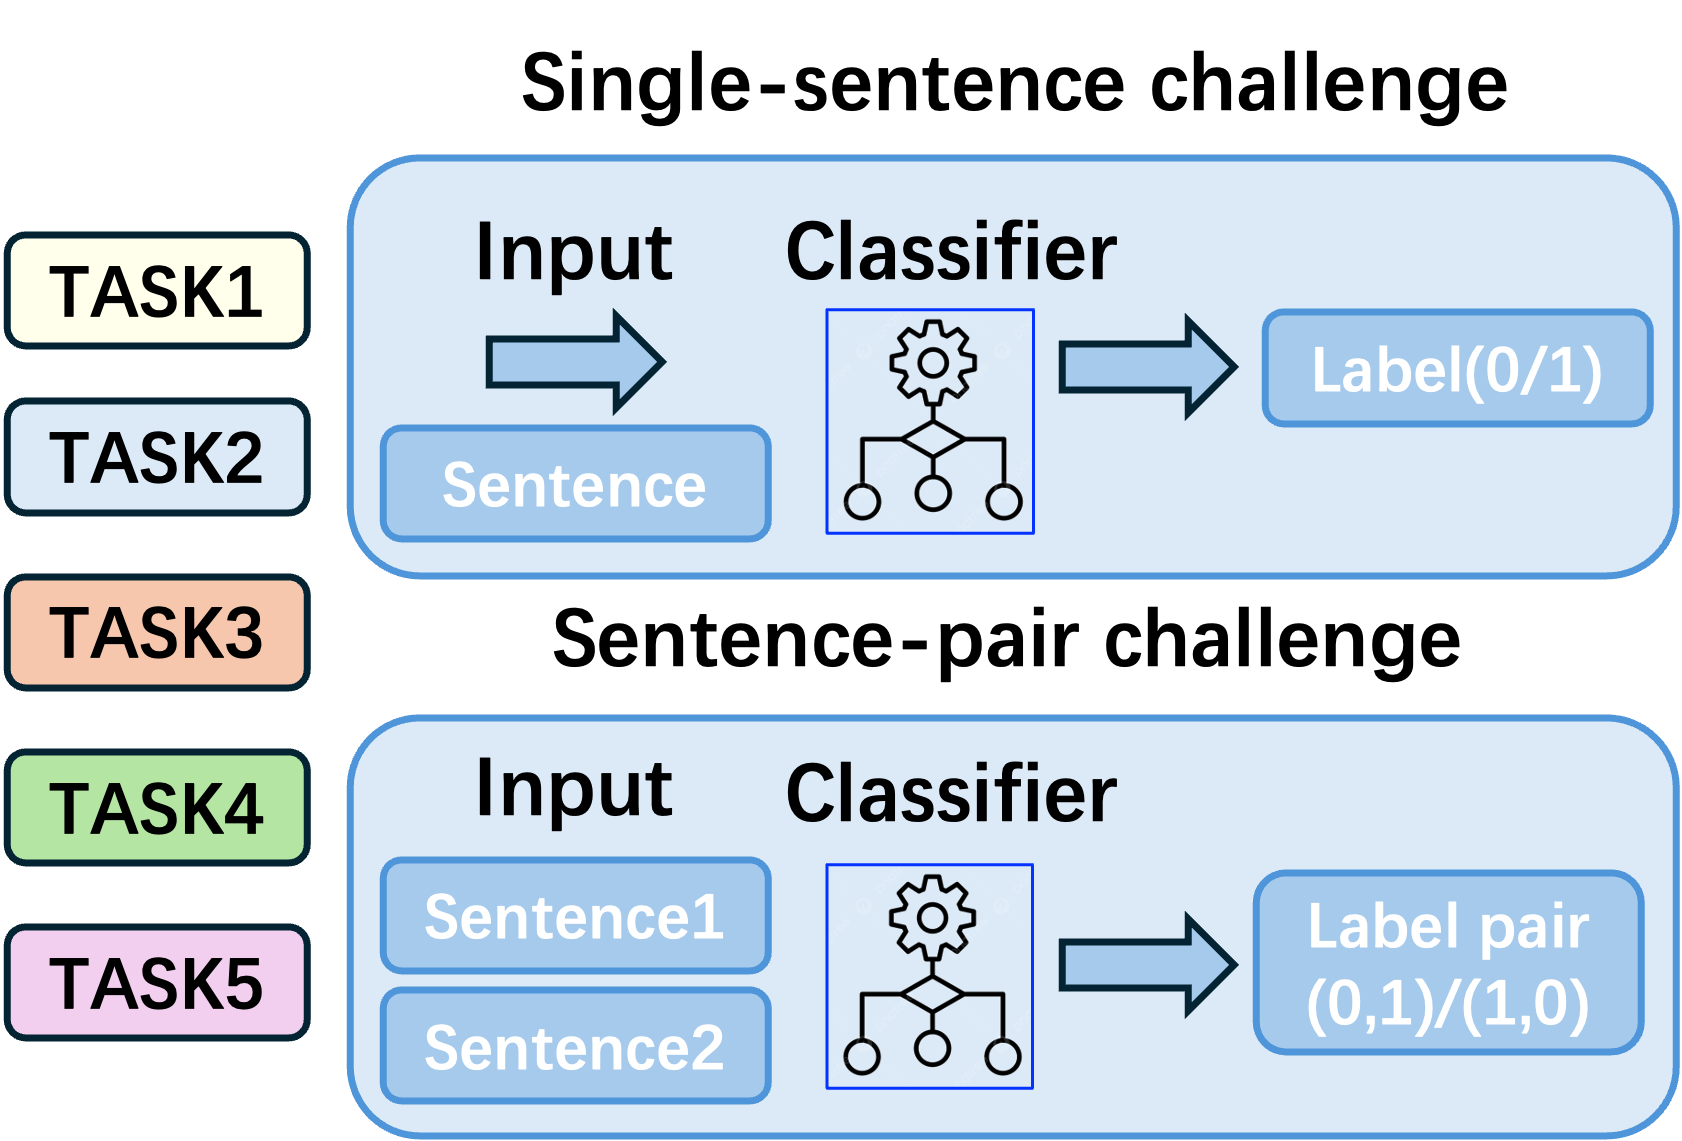
\includegraphics[width=0.82\textwidth]{figures/evaluation_setup.png}
    \caption{Two evaluation challenges: single-sentence classification and sentence-pair recognition. All five tasks are transformed into these two challenge formats.}
    \label{fig:evaluation_setup}
\end{figure}
Five distinct experimental settings, illustrated in Fig~\ref{fig:evaluation_setup}, systematically vary data utilization strategies and task formulations to provide robust evaluation frameworks.

\paragraph{Rationale for Five-Setting Framework.} The framework addresses fundamental limitations through systematic variation of three critical dimensions:\\
(1) \textbf{Data Utilization Strategy}: Exhaustive vs.\ sampling approaches to control semantic repetition;\\
(2) \textbf{Label Distribution}: Balanced vs.\ imbalanced scenarios to test base rate sensitivity;\\
(3) \textbf{Task Formulation}: Absolute vs.\ comparative classification paradigms.

\subsection{Setting 1: Single-Sentence Exhaustive Method}
\label{appD:setup_1}
The exhaustive method implements a comprehensive data utilization strategy where all available instances from both relevant text types are used to create the maximum possible dataset size. Algorithm~\ref{algo:exhaustive_method} shows the technical specifics.

\paragraph{Characteristics.} Dataset size: $2\times$ original size (e.g., 16,233 $\to$ 32,466 samples); Label distribution: Fixed 50-50 balance; Data utilization: Exhaustive use of all available instances.

\subsection{Settings 2--4: Single-Sentence Sampling Method}
The sampling method addresses evaluation validity concerns by implementing \textbf{controlled semantic exposure}. Algorithm~\ref{algo:sampling_method} provides technical details.

\paragraph{Distribution Settings.} \textbf{Setting 2 (30-70):} Sampling probability $p = 0.3$, focusing on imbalanced dataset performance. \textbf{Setting 3 (50-50):} Sampling probability $p = 0.5$, enabling direct comparison with exhaustive method. \textbf{Setting 4 (80-20):} Sampling probability $p = 0.8$, testing detector robustness with majority LLM-generated content.

\begin{algorithm}[H]
\caption{Single-Sentence Sampling Method}
\begin{algorithmic}[1]
\label{algo:sampling_method}
\STATE \textbf{Input:} Dataset $D$ with $n$ samples, Task $(T_A, T_B)$, sampling ratio $p$
\STATE \textbf{Initialize:} $samples \leftarrow \emptyset$, random seed
\FOR{each sample $s_i \in D$}
    \STATE Generate random value $r \sim \text{Uniform}(0,1)$
    \IF{$r < p$}
        \STATE Select $text \leftarrow s_i[T_B]$, $label \leftarrow 1$
    \ELSE
        \STATE Select $text \leftarrow s_i[T_A]$, $label \leftarrow 0$
    \ENDIF
    \STATE Create sample: $(idx=i, sentence=text, label=label)$
    \STATE $samples \leftarrow samples \cup \{(i, text, label)\}$
\ENDFOR
\STATE \textbf{Output:} Dataset of size $n$ with target label distribution
\end{algorithmic}
\end{algorithm}

\subsection{Setting 5: Sentence-Pair Recognition}
\label{appD:setup5}
Sentence-pair recognition addresses a fundamental limitation in current AI text detection evaluation. Pair-wise evaluation better mirrors real-world scenarios where humans and detectors must choose between alternatives of unknown provenance.

\begin{algorithm}[H]
\caption{Sentence-Pair Recognition Challenge}
\begin{algorithmic}[1]
\STATE \textbf{Input:} Dataset $D$ with $n$ samples, Task $(T_A, T_B)$
\STATE \textbf{Initialize:} $pairs \leftarrow \emptyset$
\FOR{each sample $s_i \in D$}
    \STATE Extract $sentence_A \leftarrow s_i[T_A]$
    \STATE Extract $sentence_B \leftarrow s_i[T_B]$
    \STATE Generate random bit $flip \sim \text{Bernoulli}(0.5)$
    \IF{$flip = 0$}
        \STATE $pair \leftarrow [sentence_A, sentence_B]$, $labels \leftarrow [0, 1]$
    \ELSE
        \STATE $pair \leftarrow [sentence_B, sentence_A]$, $labels \leftarrow [1, 0]$
    \ENDIF
    \STATE Create sample: $(idx=i, sentence\_pair=pair, label\_pair=labels)$
    \STATE $pairs \leftarrow pairs \cup \{(i, pair, labels)\}$
\ENDFOR
\STATE \textbf{Output:} Dataset of $n$ sentence pairs with randomized order
\end{algorithmic}
\end{algorithm}

\subsection{Summary}

\begin{table}[t]
\centering
\caption{Comparative analysis of the five evaluation settings.}
\label{tab:setup_comparison}
\begin{tabular}{@{}lcccccc@{}}
\toprule
\textbf{Aspect} & \textbf{Exhaustive} & \textbf{30-70} & \textbf{50-50} & \textbf{80-20} & \textbf{Sentence-Pair} \\
\midrule
Dataset Size & $2n$ & $n$ & $n$ & $n$ & $n$ \\
Label Distribution & 50-50 & 30-70 & 50-50 & 80-20 & Balanced pairs \\
Semantic Repetition & Present & Eliminated & Eliminated & Eliminated & Eliminated \\
Data Utilization & Complete & Sampled & Sampled & Sampled & Complete per pair \\
Evaluation Type & Absolute & Absolute & Absolute & Absolute & Comparative \\
Bias Concerns & Semantic & Distribution & Minimal & Distribution & Positional \\
Research Focus & Max performance & Minority class & Balanced & Majority class & Comparative \\
\bottomrule
\end{tabular}
\end{table}

\section{Detailed Evaluation Settings}

\subsection{Evaluation Metrics}

\textbf{Area Under ROC Curve (AUROC):} Measures the detector's ability to distinguish between human and AI-generated text across all classification thresholds. AUROC values range from 0.5 (random performance) to 1.0 (perfect classification).

\textbf{TPR@1\%FPR:} True Positive Rate when False Positive Rate is constrained to 1\%.\\
\textbf{TPR@5\%FPR:} True Positive Rate when False Positive Rate is constrained to 5\%.\\
\textbf{TPR@10\%FPR:} True Positive Rate when False Positive Rate is constrained to 10\%.

\subsection{Zero-Shot Detectors Setup}
\label{appE:zero-shot_setup}

\subsubsection{Binoculars Configuration}
\textbf{Model Configuration:}
\begin{enumerate}[nosep]
    \item \textbf{Observer Model:} \texttt{tiiuae/falcon-7b}
    \item \textbf{Performer Model:} \texttt{tiiuae/falcon-7b-instruct}
    \item \textbf{Detection Mode:} Accuracy-optimized
\end{enumerate}

\subsubsection{GLTR Configuration}
\textbf{Model Configuration:}
\begin{enumerate}[nosep]
    \item \textbf{Primary Model:} GPT-2-large
    \item \textbf{Analysis Window:} Full text sequences up to model maximum length
\end{enumerate}

\subsubsection{Fast-DetectGPT Configuration}
\textbf{Model Configuration:}
\begin{enumerate}[nosep]
    \item \textbf{Scoring Model:} \texttt{falcon-7b-instruct}
    \item \textbf{Sampling Model:} Same as scoring model for efficiency
    \item \textbf{Sampling Parameters:} 10,000 samples for probability estimation
\end{enumerate}

The Fast-DetectGPT criterion is:
\begin{equation}
\text{Criterion} = \frac{\log p_{\theta}(x) - \mu_{\tilde{x}}}{\sigma_{\tilde{x}}}
\end{equation}
where $\mu_{\tilde{x}}$ and $\sigma_{\tilde{x}}$ are sample statistics.

\subsubsection{RADAR Configuration}
\textbf{Model Configuration:}
\begin{enumerate}[nosep]
    \item \textbf{Base Model:} RoBERTa-large (355M parameters)
    \item \textbf{RADAR Model:} TrustSafeAI/RADAR-Vicuna-7B
    \item \textbf{Input Processing:} Maximum sequence length of 512 tokens
\end{enumerate}

The detection score is:
\begin{equation}
P(\text{AI-generated}) = \exp(\log\text{-softmax}(\text{logits})_0)
\end{equation}

\subsection{Model-Based Detectors Setup}

\textbf{Model Selection:} Claude-3.5-Haiku, DeepSeek-V2.5, Gemma-3-27B, Llama-4-Scout-17B, Mistral-Nemo, Llama-4-Maverick-17B, WizardLM-2-8x22B

\textbf{Prompt Engineering Strategy:}
\begin{enumerate}
    \item \textbf{System Message:} Establishes expert persona and task context
    \item \textbf{Few-Shot Examples:} 3--4 carefully crafted demonstrations per task
    \item \textbf{Multi-Turn Conversation:} Maintains context across examples
    \item \textbf{Task-Specific Expertise:} Specialized personas for different detection tasks
\end{enumerate}

\paragraph{Single-Sentence Classification Prompt Templates:}
\label{appE:single-sentence_model_prompting}

\noindent \textbf{Task 1 --- Paraphrase Source Attribution:}
\begin{quote}
\itshape
``You are an expert text analyst specializing in paraphrase detection. Your task is to determine whether a paraphrased sentence was created by a human or by an AI/LLM system.

CLASSIFICATION CRITERIA:
- Human paraphrase (0): Natural flow, contextual understanding, human-like word choices
- LLM paraphrase (1): Systematic rewording patterns, over-precision, AI-like formalization

IMPORTANT: You must respond with ONLY the number 0 or 1.''
\end{quote}

\noindent \textbf{Task 2 --- General Text Authorship Detection:}
\begin{quote}
\itshape
``You are an expert in AI-generated text detection. Determine whether a sentence was originally written by a human or generated by an AI/LLM system.

CLASSIFICATION CRITERIA:
- Human original (0): Authentic voice, natural imperfections, personal style
- LLM generated (1): Training data patterns, generic expressions, artificial smoothness

IMPORTANT: You must respond with ONLY the number 0 or 1.''
\end{quote}

\noindent \textbf{Task 3 --- AI Text Laundering Detection:}
\begin{quote}
\itshape
``You are a specialist in detecting AI text laundering techniques. Determine the level of AI processing in text --- distinguishing LLM-paraphrased original content versus LLM-paraphrased generated content.

CLASSIFICATION CRITERIA:
- LLM paraphrased original (0): AI paraphrase of human content
- LLM paraphrased generated (1): AI paraphrase of AI content --- multiple layers of AI processing

IMPORTANT: You must respond with ONLY the number 0 or 1.''
\end{quote}

\noindent \textbf{Task 4 --- Iterative Paraphrase Depth Detection:}
\begin{quote}
\itshape
``You are an expert in detecting iterative AI processing depth. Determine whether text has undergone fewer or more iterations of LLM paraphrasing.

CLASSIFICATION CRITERIA:
- 1st iteration paraphrase (0): Less deep AI processing
- 3rd iteration paraphrase (1): Deeper AI processing, heavily transformed

IMPORTANT: You must respond with ONLY the number 0 or 1.''
\end{quote}

\noindent \textbf{Task 5 --- Deep Paraphrase Attack Detection:}
\begin{quote}
\itshape
``You are a cybersecurity expert specializing in detecting sophisticated AI paraphrase attacks. Distinguish between authentic human-written text and heavily processed AI paraphrases.

CLASSIFICATION CRITERIA:
- Human original (0): Authentic human expression, natural imperfections
- Deep paraphrase attack (1): Heavily processed AI text, multiple transformation layers

IMPORTANT: You must respond with ONLY the number 0 or 1.''
\end{quote}

\paragraph{Sentence-Pair Comparative Prompting:}
For sentence-pair tasks, the prompting strategy shifts to comparative analysis where models must determine which sentence in a pair exhibits more human-like or AI-like characteristics. Corresponding comparative versions of the above system messages are used for each task, instructing the model to respond with 0 if the first sentence is more human-like, and 1 if the second sentence is more human-like.

\noindent \textbf{Multi-Turn Conversation Structure:}

Each evaluation follows a consistent multi-turn conversation pattern:
\begin{enumerate}
    \item \textbf{System Message:} Task-specific expert persona and classification criteria
    \item \textbf{Few-Shot Example 1--3:} User query with example text $\to$ Assistant response with label
    \item \textbf{Target Query:} User query with actual text to classify $\to$ Assistant response (evaluated)
\end{enumerate}

\section{Ethics Statements and Limitations}

\subsubsection{Ethics Statement}
Only publicly available datasets and pre-trained models are used in this study, accessed and utilized strictly for research purposes. The use of these resources complies with their original licenses and terms of access. No personally identifiable or sensitive information is present in any of the data used.

The code will be released under the MIT license to support transparency and reproducibility.

\subsubsection{Limitations}

While PADBen provides comprehensive evaluation of paraphrase attack robustness, several aspects could be enhanced in future iterations:

\textbf{Experimental Controls.} The Experiment 2 trajectory analysis could benefit from stricter variable control, particularly maintaining consistent text length across paraphrasing iterations and expanding sample sizes beyond 100 texts per category.

\textbf{Taxonomy Coverage.} The five-type taxonomy focuses on core paraphrase attack scenarios but could expand to include additional variants, specifically extending Type 5 beyond 3 iterations and introducing intermediate iteratively-paraphrased human texts variants.

\textbf{Detector Optimization.} Zero-shot detectors are evaluated using default configurations without fine-tuning on PADBen data. While this approach assesses out-of-the-box robustness, adapted implementations could potentially improve performance.

\textbf{Evaluation Comprehensiveness.} Current sentence-pair tasks exclusively include paraphrased text in at least one position. Incorporating additional pairs without paraphrasing would provide more diverse evaluation scenarios.

These limitations represent opportunities for enhancement rather than fundamental flaws. PADBen's current design prioritizes realistic attack scenarios, mechanistic insights, and comprehensive detector evaluation within practical resource constraints.
